\documentclass[10pt]{beamer}
\usepackage{../sty/phylo-csntm-talk}
\definecolor{Bluesky}{RGB}{0,128,255}
\title{Phylogenetics\\and the CBGM\\@ CSNTM}
\subtitle{Center for the Study of New Testament Manuscripts\\12 February 2024}
\author{Joey McCollum}
\institute{Australian Catholic University\\Institute for Religion and Critical Inquiry\\ \faEnvelope\quad\href{mailto:james.mccollum@myacu.edu.au}{james.mccollum@myacu.edu.au}\\ \faTwitter\quad @JoeyMcCollum\\ \faGithub\quad\href{https://github.com/jjmccollum}{jjmccollum}}
\date{} % insufficient space on this side, so move under subtitle
\begin{document}
	\begin{frame}
		\titlepage
	\end{frame}
	\section{Preliminaries}
	\subsection{Collation}
	\begin{frame}
		\begin{itemize}
			\item To compare textual witnesses, align them at independent \emph{variation units}
			\item \emph{Variant readings} occur at variation units
		\end{itemize}
		\begin{center}
			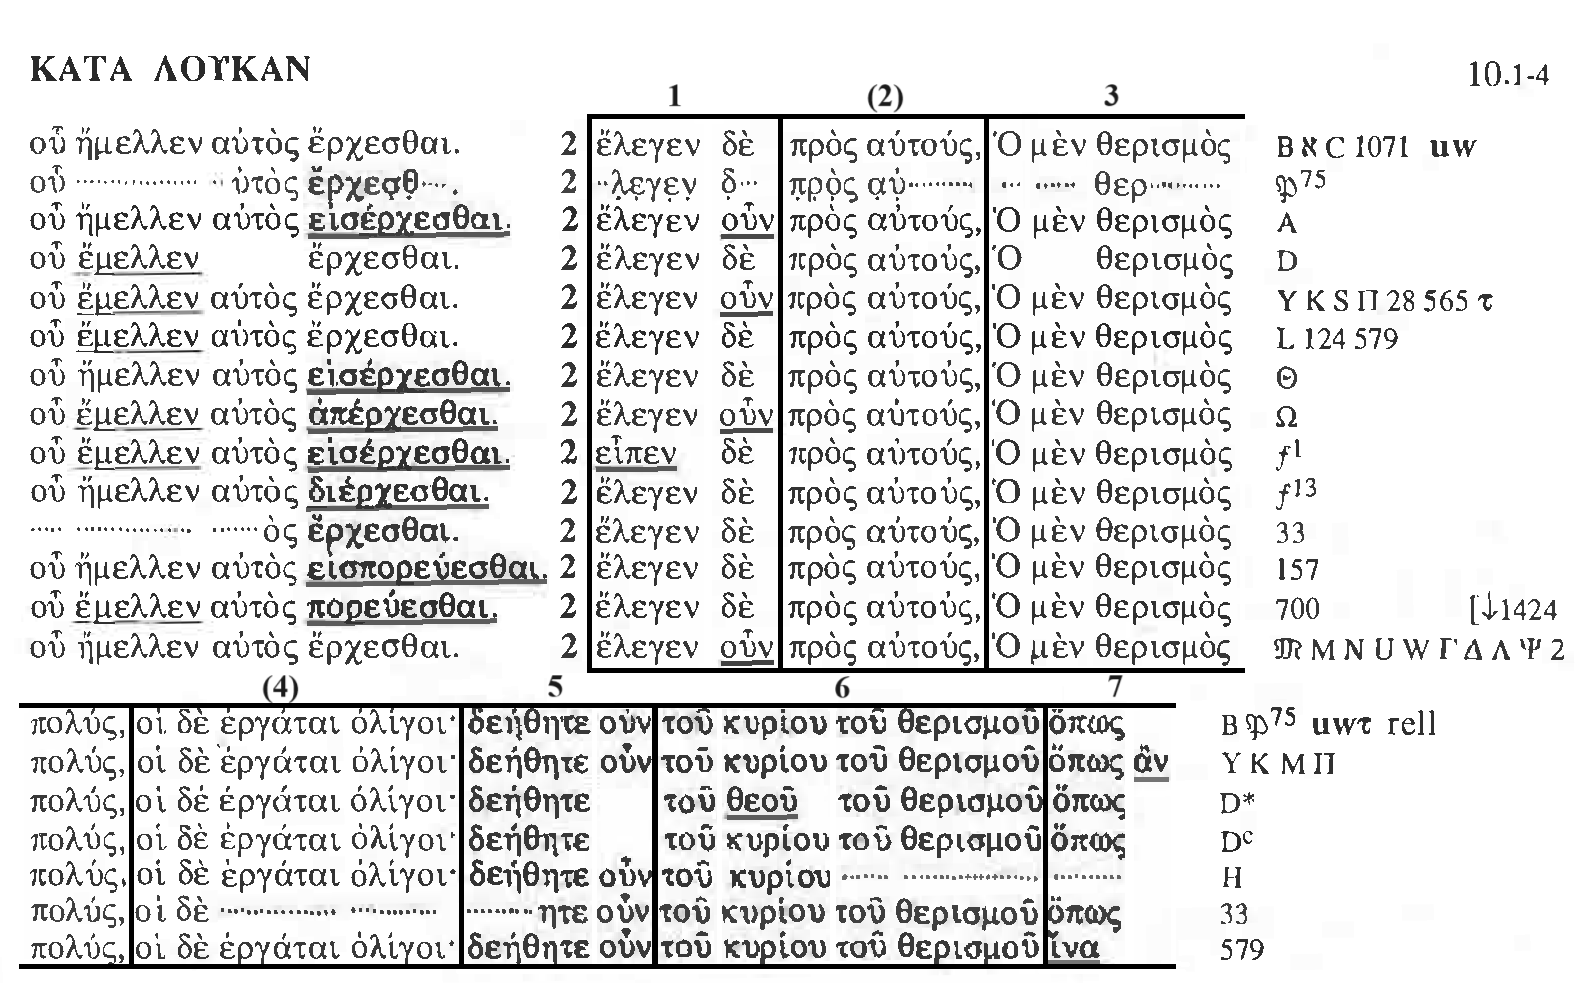
\includegraphics[width=0.75\textwidth]{../img/swanson-luke-10-2-variation-units.png}
		\end{center}
		\footnotesize Collation of Luke 10:2 with variation units numbered above text \parencite[Source:][183]{Swanson.Luke}
	\end{frame}
	\begin{frame}
		\begin{itemize}
			\item Analogous to a DNA sequence alignment
		\end{itemize}
		\begin{center}
			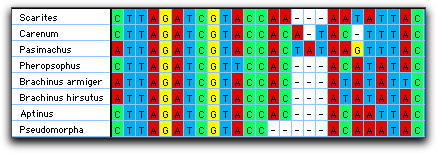
\includegraphics[scale=0.5]{../img/sequence-alignment.jpg}
		\end{center}
		\begin{itemize}
			\item Rows: \emph{taxa} = witnesses
			\item Columns: \emph{sites} = variation units
			\item Cells: \emph{states} = variant readings (including omissions)
			\begin{itemize}
				\item Lacunae and uncertain retroversions correspond to fully or partially \emph{ambiguous states}
			\end{itemize}
		\end{itemize}
	\end{frame}
	\subsection{Witnesses}
	\begin{frame}
		\begin{itemize}
			\item At the most basic level, a \emph{witness} is just a sequence of readings, a row in the collation
		\end{itemize}
		\begin{center}
			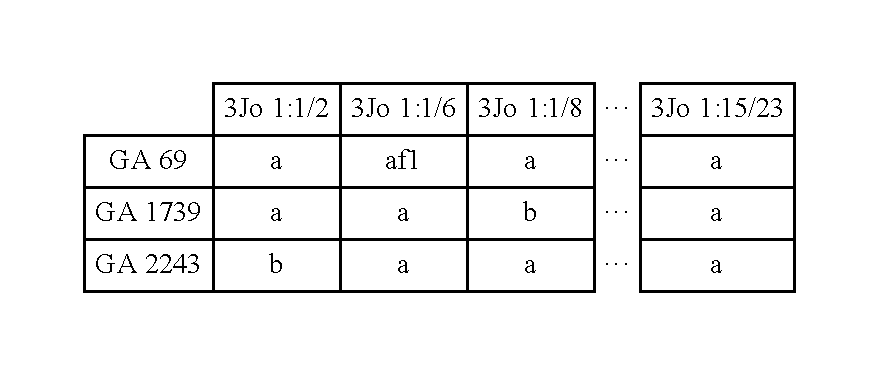
\includegraphics[scale=0.5]{../img/witnesses.pdf}
		\end{center}
		\begin{itemize}
			\item Paratextual features can be encoded in the same way
			\item In more complex phylogenetic approaches, age can also be incorporated
		\end{itemize}
	\end{frame}
	\section{Phylogenetics}
	\subsection{Fundamentals}
	\begin{frame}
		\begin{center}
			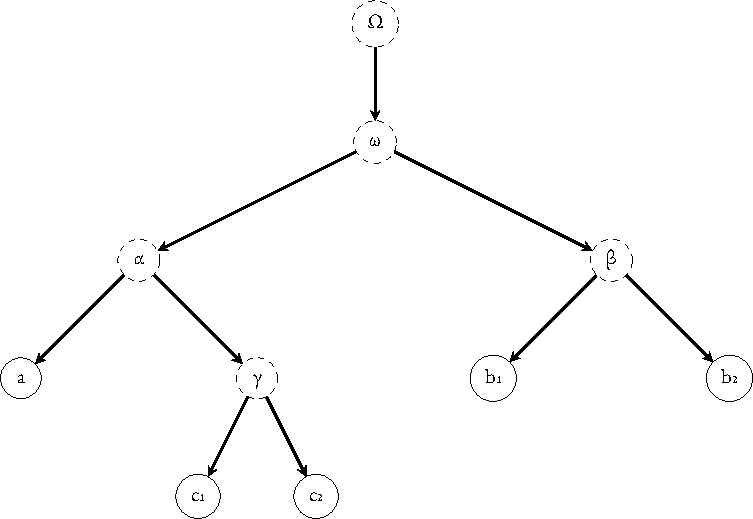
\includegraphics[scale=0.5]{../img/gene-tree-rooted-site-1.pdf}
		\end{center}
		\begin{itemize}
			\item A \emph{stemma} is a \textquote{family tree} modeling the transmission of the text
			\item The \emph{leaves} (solid circles) correspond to extant witnesses
			\item The \emph{hyparchetypes} (dashed circles) are hypothetical (now-lost) ancestors, reconstructed from their descendents along the branches
			\item The \emph{archetype} (\textgreek{ω}) is the earliest reconstructible text
			\item The \emph{root} (\textgreek{Ω}) represents the authorial text
		\end{itemize}
	\end{frame}
	\begin{frame}
		\begin{tabular}{p{0.4\textwidth} @{\hskip 0.2\textwidth} p{0.4\textwidth}}
			\vspace{0pt}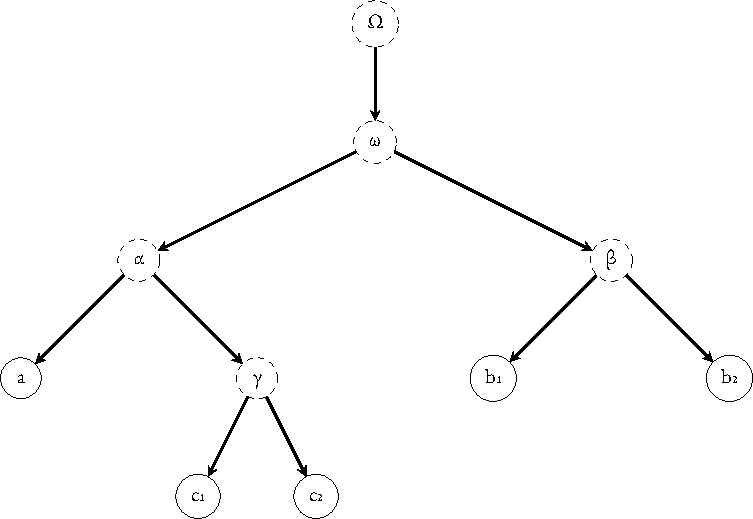
\includegraphics[scale=0.4]{../img/gene-tree-rooted-site-1.pdf} & \vspace{0pt}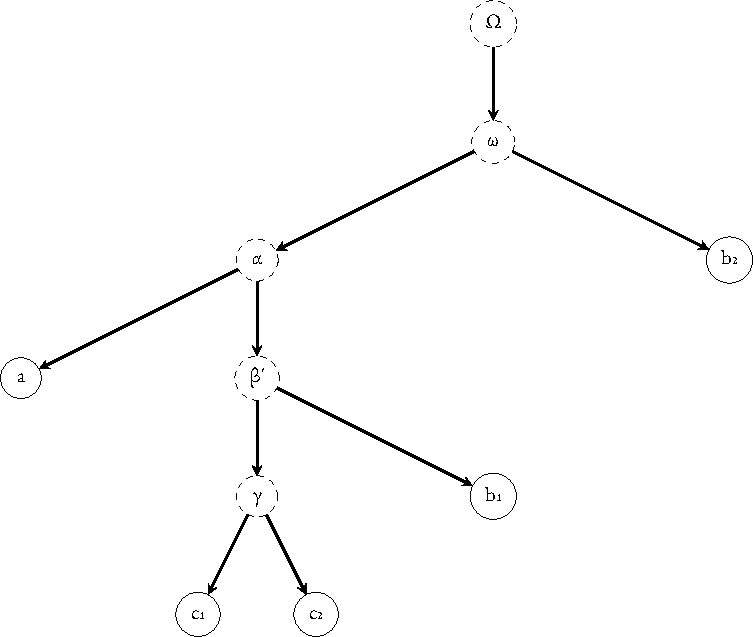
\includegraphics[scale=0.4]{../img/gene-tree-rooted-site-2.pdf}
		\end{tabular}
		\begin{itemize}
			\item A stemma represents a hypothesis about transmission history
			\item The goal is to determine which hypothesis (or hypotheses) best explain the extant data
			\item To do this, we need a numerical metric or \textquote{score} for the fitness of a given stemma
		\end{itemize}
	\end{frame}
	\subsection{Parsimony}
	\begin{frame}
		\begin{itemize}
			\item One such metric is \emph{parsimony}
			\item The smallest number of times one reading has to change to another along the branches of the stemma
			\item Motivated by Ockham's Razor
			\item Given a candidate stemma, we calculate its parsimony score for each variation unit independently, then add up the results
			\item Can be efficiently computed in a bottom-up fashion
		\end{itemize}
		\begin{center}
			\setmainfont[Ligatures=Common]{EB Garamond}
			\renewfontfamily\greekfont[Script=Greek]{EB Garamond}
			\begin{tabular}{|l|l|}
				\hline
				Witness & Reading\\
				\hline
				\hline
				a & {\color{red}\textgreek{χριστου ιησου}}\\
				\hline
				b\textsubscript{1} & {\color{blue}\textgreek{ιησου χριστου}}\\
				\hline
				b\textsubscript{2} & {\color{blue}\textgreek{ιησου χριστου}}\\
				\hline
				c\textsubscript{1} & {\color{darkgreen}\textgreek{χριστου}}\\
				\hline
				c\textsubscript{2} & {\color{red}\textgreek{χριστου ιησου}}\\
				\hline
			\end{tabular}
		\end{center}
	\end{frame}
	\begin{frame}
		\begin{center}
			Cost for stemma 1: \only<2-3>{\textbf{2}}\\
			\vspace{\baselineskip}
			\only<1>{
				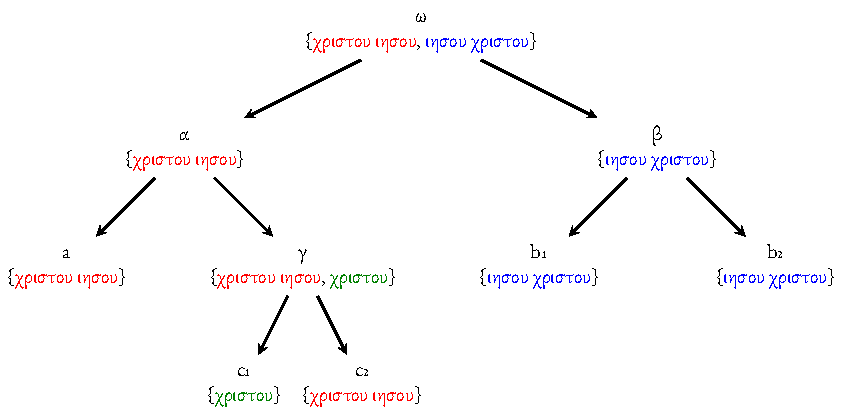
\includegraphics[scale=0.75]{../img/gene-tree-unrooted-forward-topology-1.pdf}
			}
			\only<2>{
				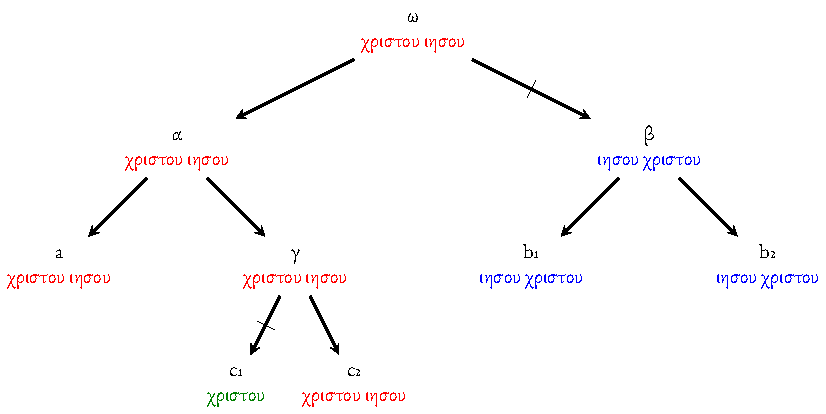
\includegraphics[scale=0.75]{../img/gene-tree-unrooted-backward-topology-1-option-1.pdf}
			}
			\only<3>{
				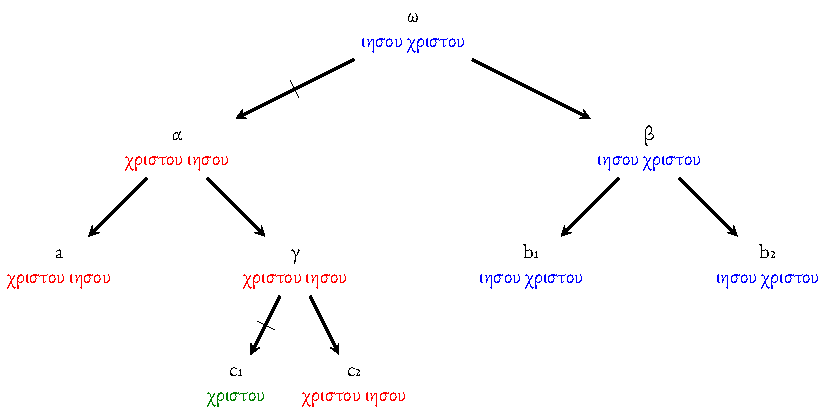
\includegraphics[scale=0.75]{../img/gene-tree-unrooted-backward-topology-1-option-2.pdf}
			}
		\end{center}
	\end{frame}
	\begin{frame}
		\begin{center}
			Cost for stemma 2: \only<2-3>{\textbf{3}}\\
			\vspace{\baselineskip}
			\only<1>{
				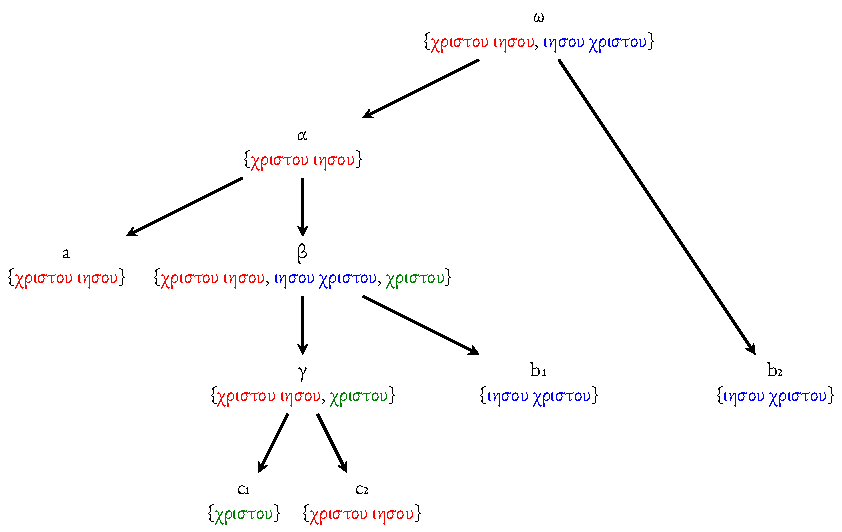
\includegraphics[scale=0.75]{../img/gene-tree-unrooted-forward-topology-2.pdf}
			}
			\only<2>{
				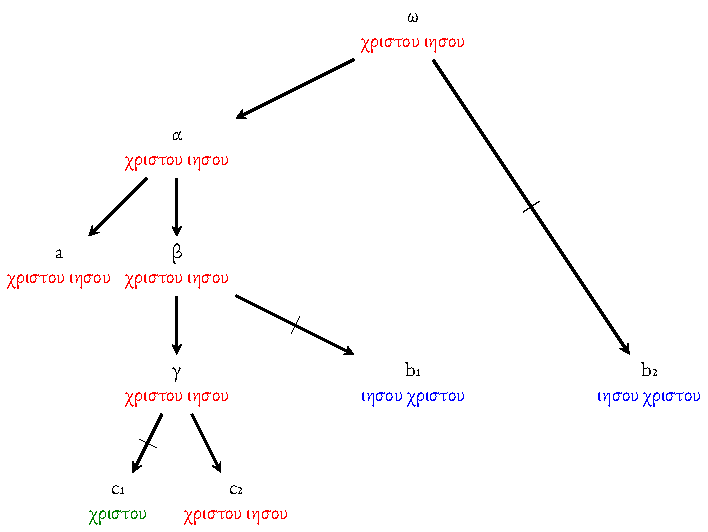
\includegraphics[scale=0.75]{../img/gene-tree-unrooted-backward-topology-2-option-1.pdf}
			}
			\only<3>{
				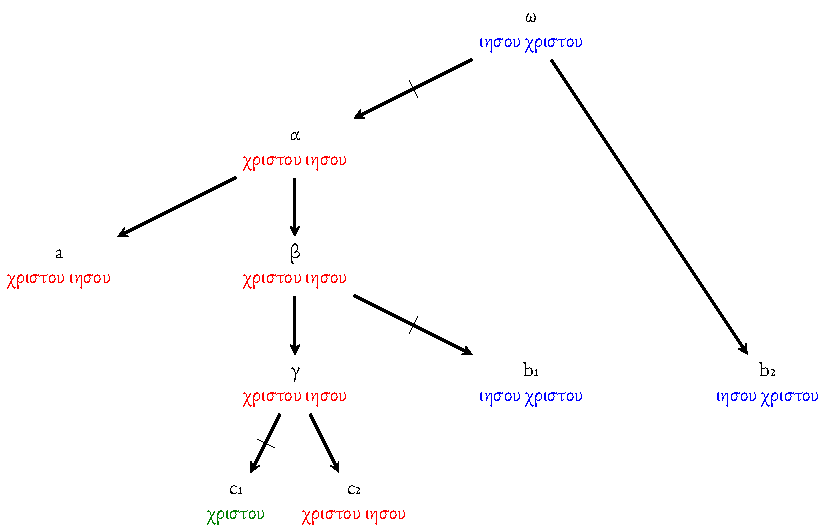
\includegraphics[scale=0.75]{../img/gene-tree-unrooted-backward-topology-2-option-2.pdf}
			}
		\end{center}
	\end{frame}
	\section{CBGM}
	\subsection{Fundamentals}
	\begin{frame}
		\begin{itemize}
			\item Developed over thirty years by Gerd Mink, culminating in the latest updates to the \emph{Editio Critica Maior} (\emph{ECM})
			\item Important reading:
			\begin{itemize} 
				\item \cite{Mink04}
				\item \cite{Gurry17}
				\item \cite{WG17}
				\item \cite{Edmondson19}
			\end{itemize}
		\end{itemize}
	\end{frame}
	\begin{frame}
		\begin{itemize}
			\item \emph{Not} a way to make computers do textual criticism, but a way for them to help us refine our judgments
			\item \emph{Not} a new methodology for evaluating variant readings, but a \textquote{meta-approach} to be used on top of existing methods
		\end{itemize}
	\end{frame}
	\begin{frame}
		\begin{itemize}
			\item Intended to solve \emph{contamination}, or mixture across branches of the textual tradition
		\end{itemize}
		\begin{center}
			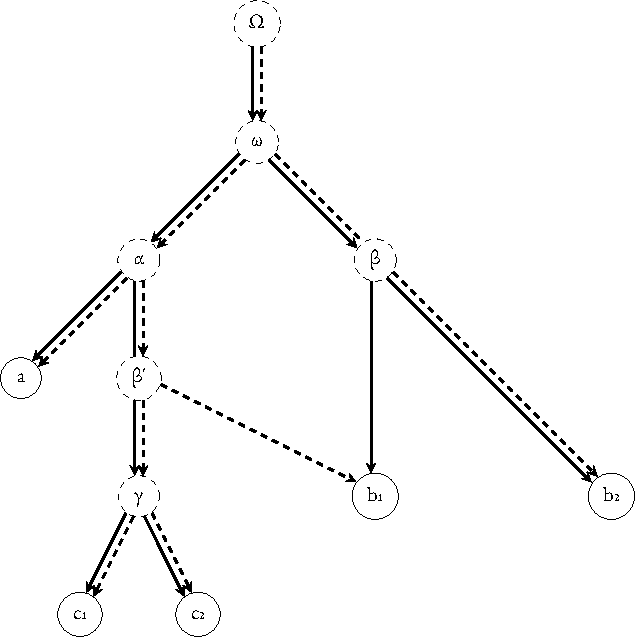
\includegraphics[scale=0.5]{../img/stemma-rooted-contamination.pdf}
		\end{center}
	\end{frame}
	\begin{frame}
		\begin{itemize}
			\item Foundational principles:
			\begin{enumerate}
				\item Scribes typically copied their exemplars with fidelity.
				\item If a scribe introduced a variant, then it came from some other reading.
				\item Scribes typically used fewer sources rather than many.
				\item Scribes typically used closely related sources rather than distant ones.
			\end{enumerate}
			\item Witnesses are \emph{texts} (sequences of readings) minus the material baggage (date, provenance, etc.)
			\begin{itemize}
				\item \textquote{How texts relate} $\neq$ \textquote{How manuscripts relate}
			\end{itemize}
		\end{itemize}
	\end{frame}
	\subsection{Local Stemmata}
	\begin{frame}
		\begin{itemize}
			\item The basic unit of comparison
			\item One for each variation unit
			\item A graphical representation of our judgments of readings
		\end{itemize}
		\begin{columns}
			\begin{column}{0.45\textwidth}
				\begin{center}
					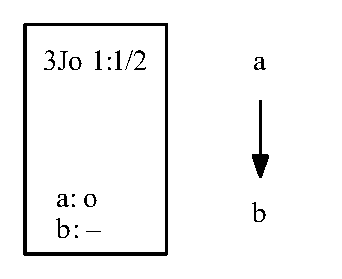
\includegraphics[scale=0.5]{../img/B25K1V1U2-local-stemma.pdf}
				\end{center}
			\end{column}
			\begin{column}{0.45\textwidth}
				\begin{center}
					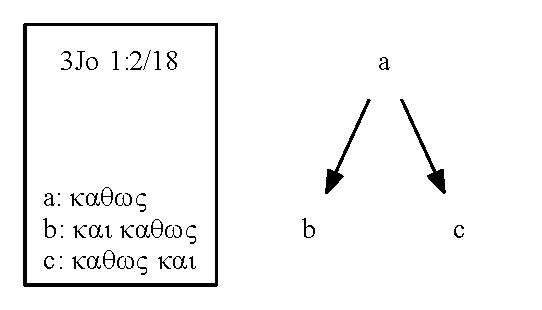
\includegraphics[scale=0.5]{../img/B25K1V2U18-local-stemma.pdf}
				\end{center}
			\end{column}
		\end{columns}
	\end{frame}
	\begin{frame}
		\begin{itemize}
			\item Some are more complicated
			\begin{itemize}
				\item \emph{defective} readings (e.g., obvious misspellings)
				\item \emph{orthographic} readings (e.g., regional differences)
				\item \emph{split} attestations of the same reading (coincidental agreement)
				\item \emph{ambiguous} readings
			\end{itemize}
			\item Some of these may be collapsed with other substantive readings
			\begin{center}
				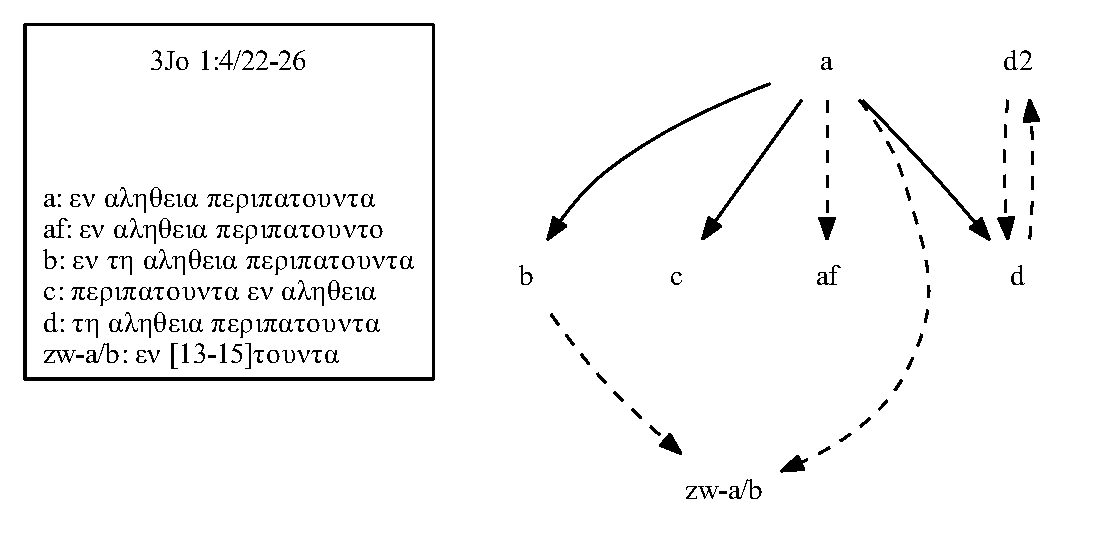
\includegraphics[scale=0.5]{../img/B25K1V4U22-26-local-stemma-ignore-defective-ignore-ambiguous-merge-splits.pdf}
			\end{center}
		\end{itemize}
	\end{frame}
	\subsection{Genealogical Relationships}
	\begin{frame}
		\begin{itemize}
			\item The relationship of two witnesses is the overall pattern \emph{of the relationships of their readings} at all variation units where both are extant
		\end{itemize}
		\begin{center}
			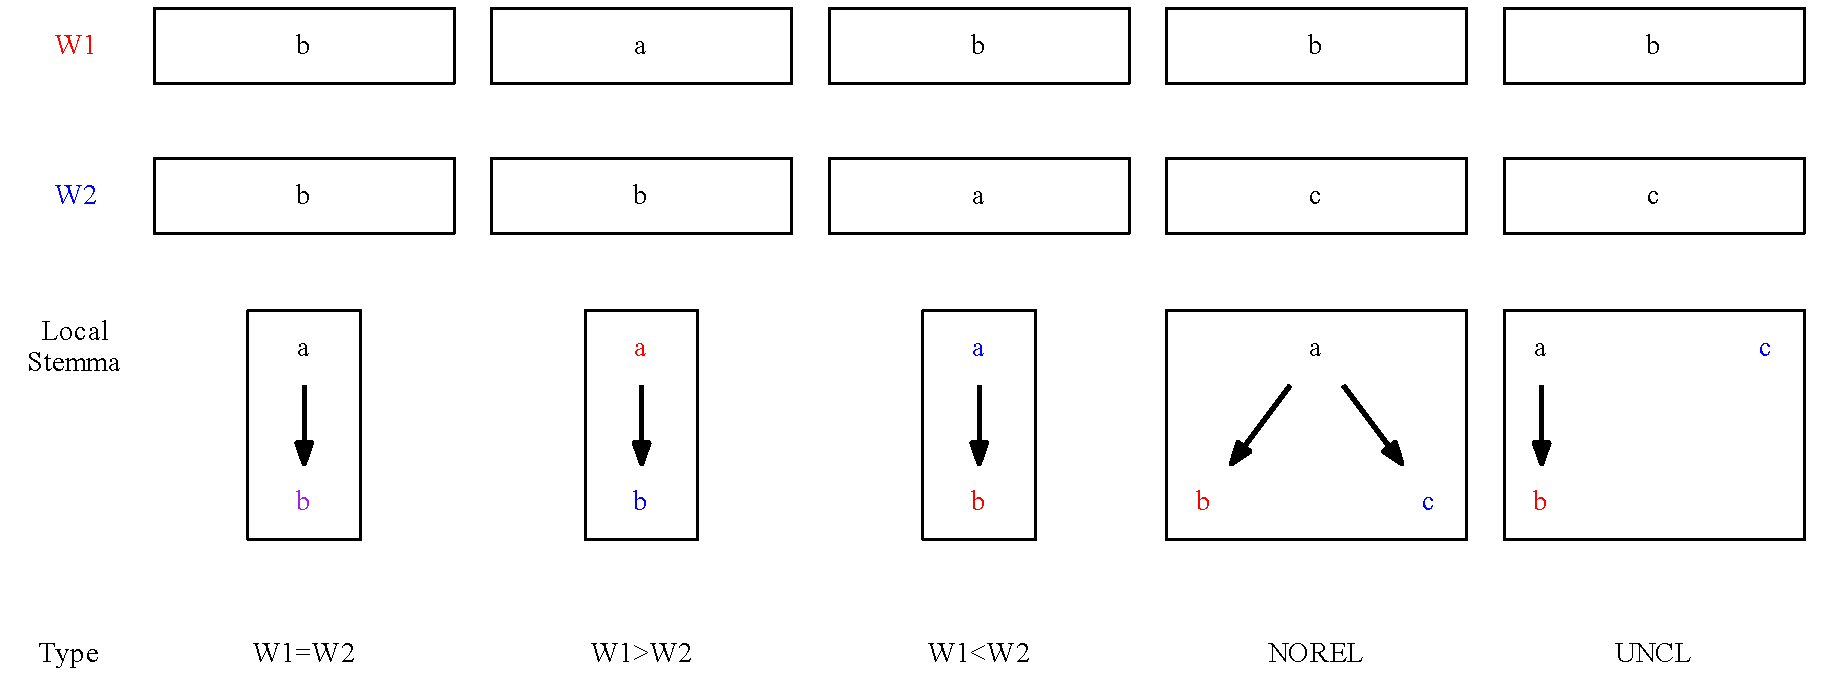
\includegraphics[width=\textwidth]{../img/genealogical-relationships.pdf}
		\end{center}
		\begin{itemize}
			\item The first three are the most important
		\end{itemize}
	\end{frame}
	\subsection{Potential Ancestors}
	\begin{frame}
		\begin{itemize}
			\item Potential ancestor = \textquote{more prior than posterior readings}
		\end{itemize}
		\begin{center}
			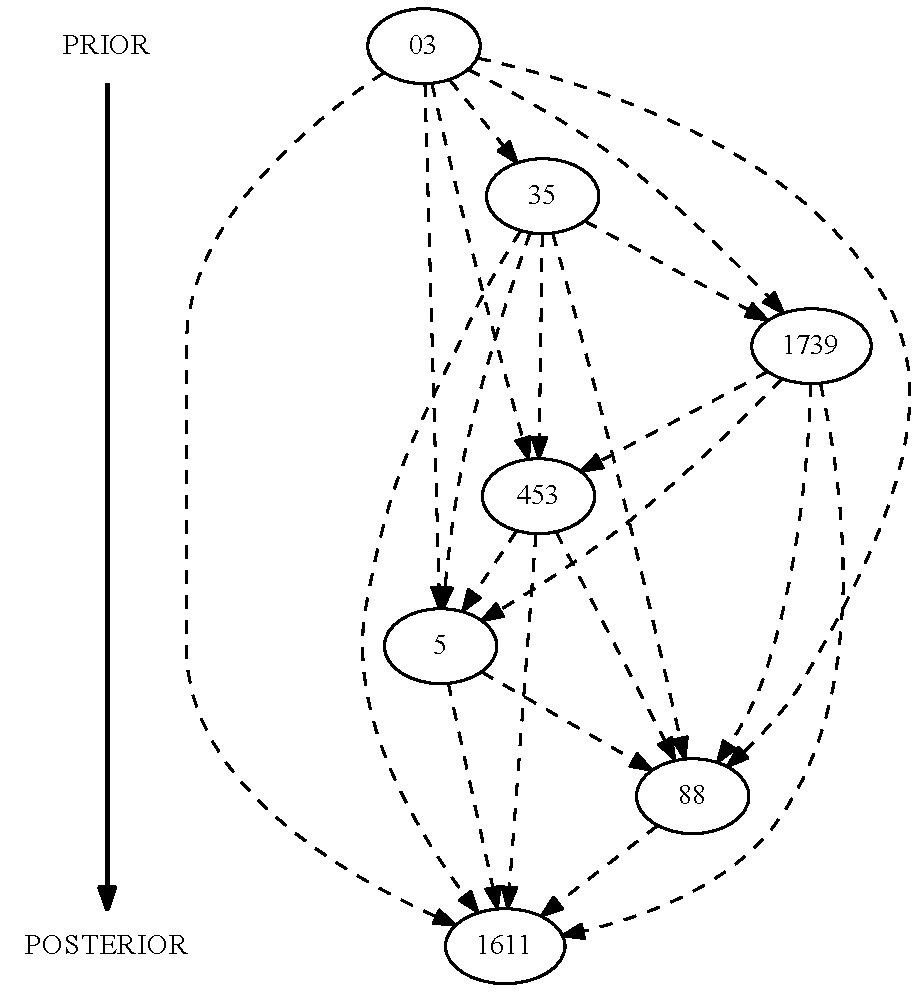
\includegraphics[scale=0.3333]{../img/potential-ancestors.pdf}
		\end{center}
	\end{frame}
	\subsection{Textual Flow}
	\begin{frame}
		\begin{columns}
			\begin{column}{0.45\textwidth}
				\begin{itemize}
					\item \emph{Textual flow} is a useful tool for helping us revise our judgments in a local stemma
					\item \emph{Not} a global stemma (our ultimate goal), but still important
				\end{itemize}
			\end{column}
			\begin{column}{0.45\textwidth}
				\begin{center}
					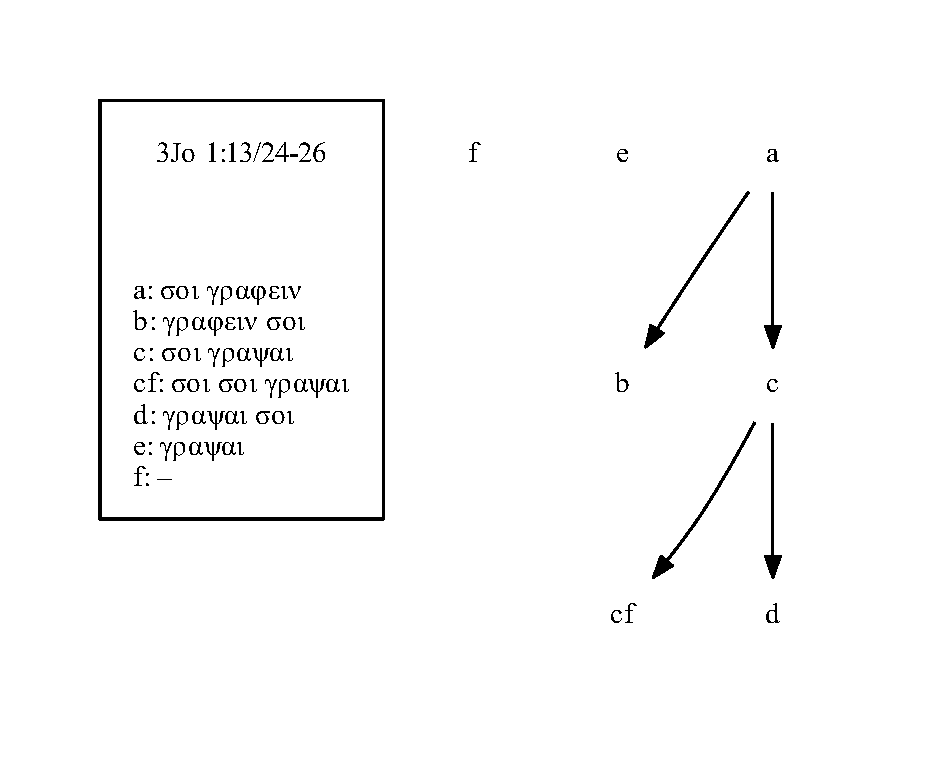
\includegraphics[width=\textwidth]{../img/B25K1V13U24-26-local-stemma-incomplete.pdf}
				\end{center}
			\end{column}
		\end{columns}
		\begin{center}
			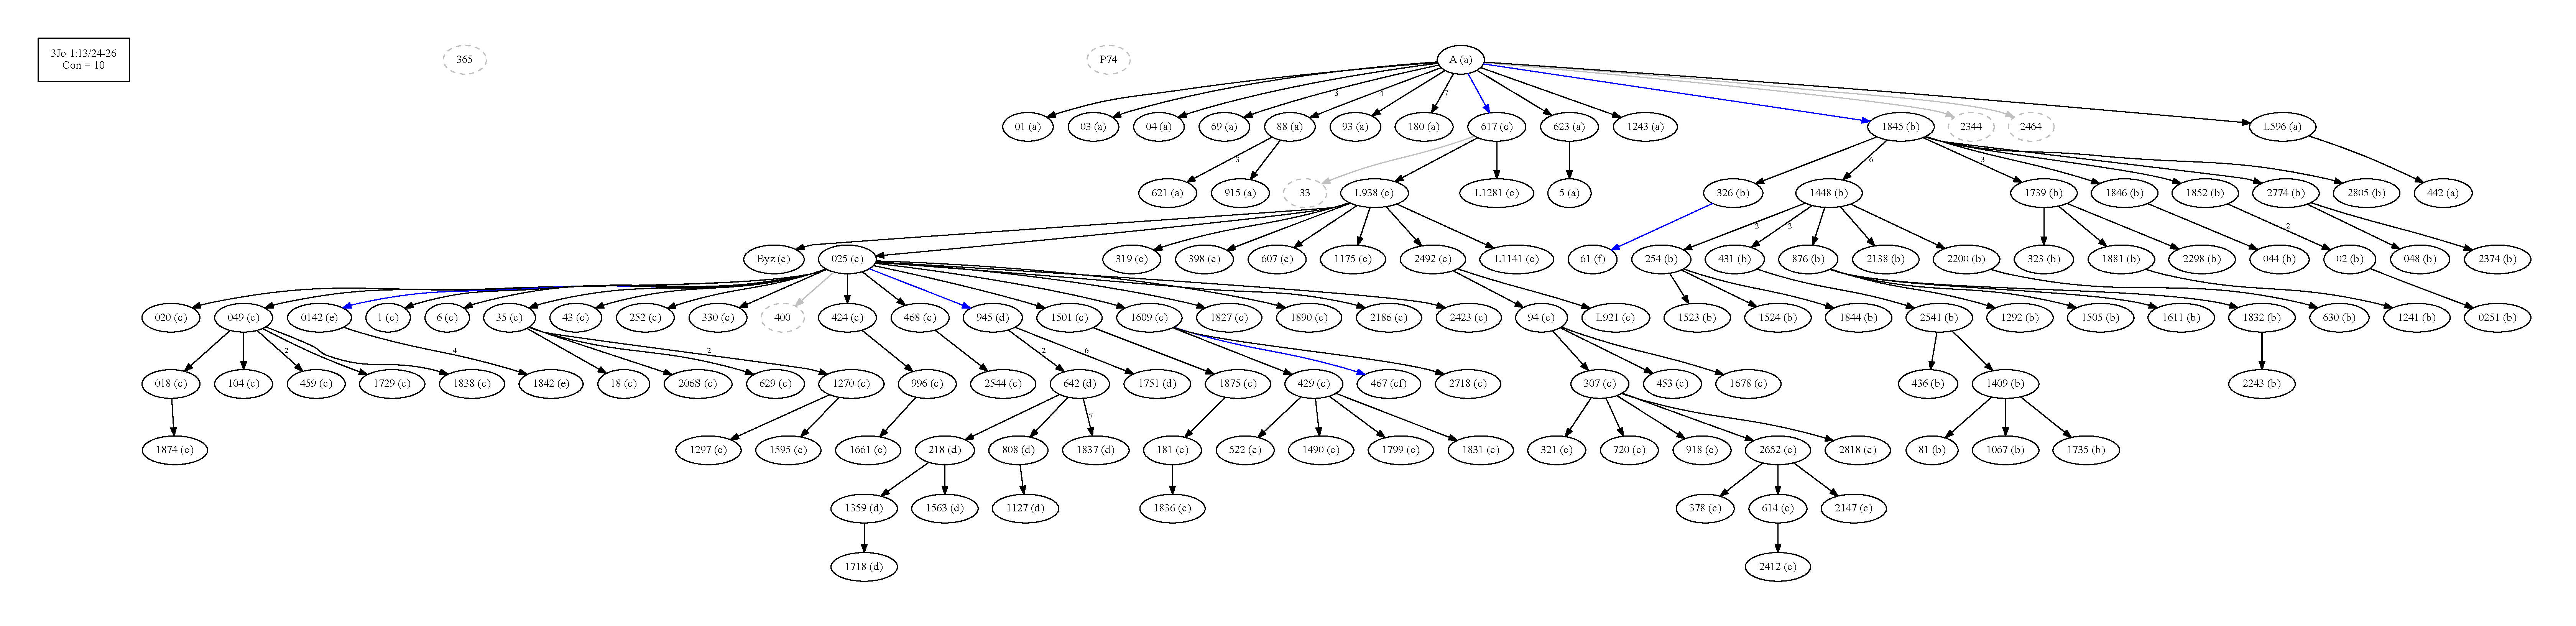
\includegraphics[width=\textwidth]{../img/B25K1V13U24-26-textual-flow.pdf}
		\end{center}
	\end{frame}
	\begin{frame}
		\begin{itemize}
			\item How do we find a given witness's \emph{textual flow ancestor}?
			\item We specify a \emph{connectivity limit} $\kappa$ (i.e., a radius of \textquote{close-enough} neighbors)
			\item Then, for each witness:
			\begin{enumerate}
				\item List its potential ancestors, sorted from most agreement to least
				\item If one of the first $\kappa$ has the same reading at this unit, then select it
				\item If not, then choose the first (non-lacunose) potential ancestor
			\end{enumerate}
			\item Core idea: use \emph{general relationships} (between witnesses) to find \emph{specific relationships} (between readings in a local stemma)
		\end{itemize}
	\end{frame}
	\begin{frame}
		\begin{itemize}
			\item Often, we just want to know the textual flow for witnesses with a specific reading
		\end{itemize}
		\begin{center}
			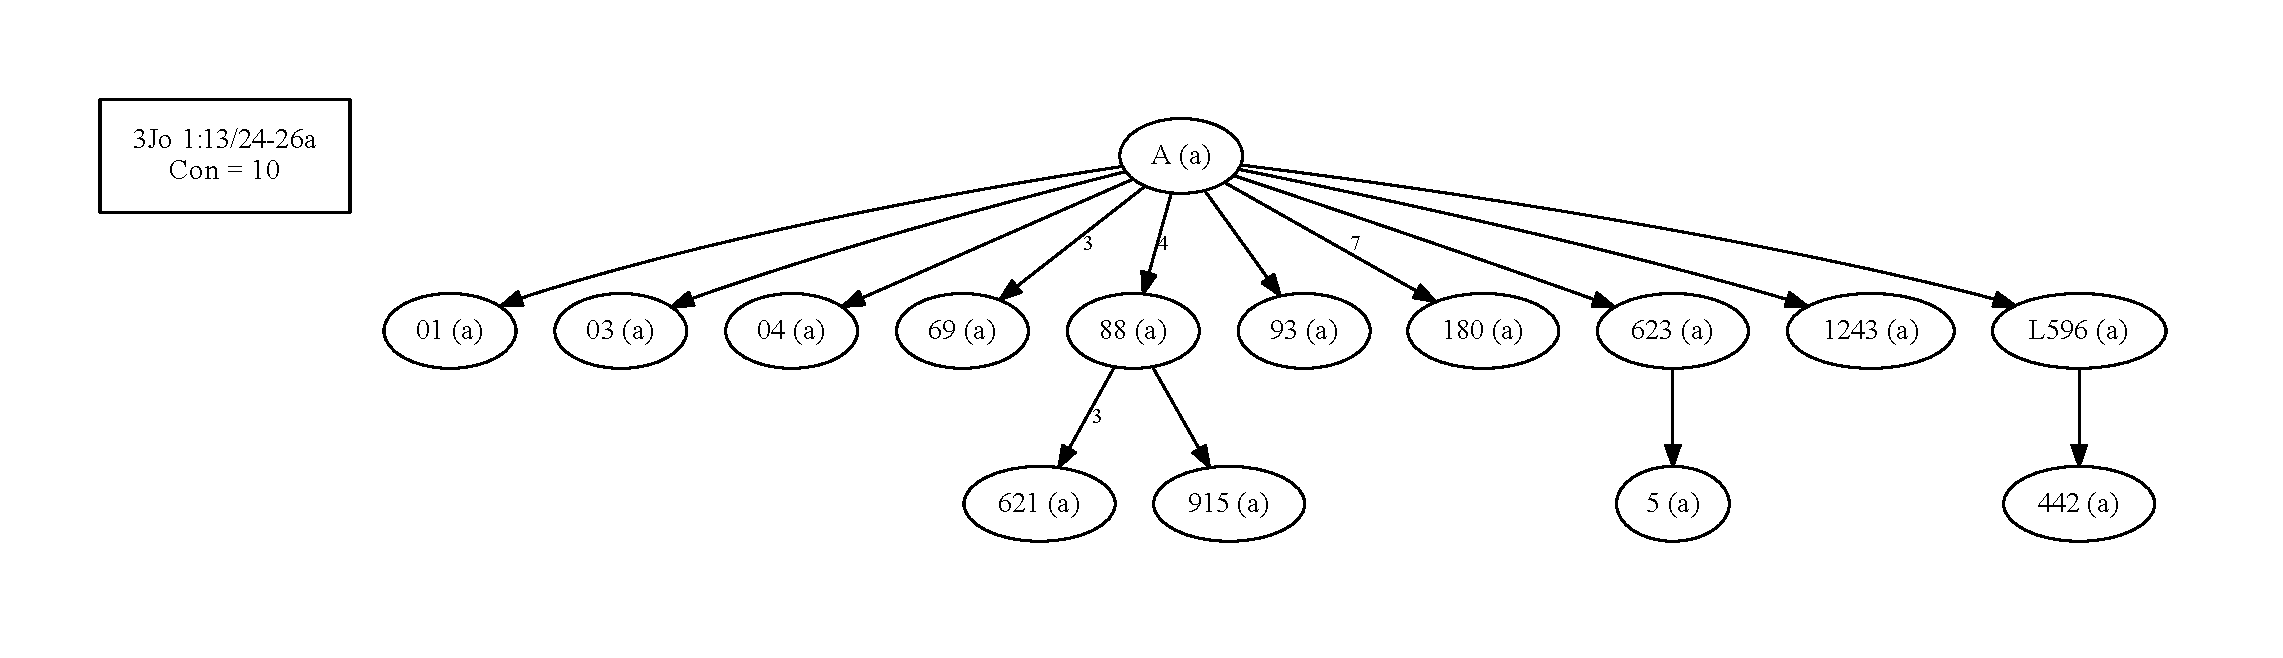
\includegraphics[width=\textwidth]{../img/B25K1V13U24-26Ra-coherence-attestations.pdf}
		\end{center}
		\begin{itemize}
			\item (Numbers on edges represent the rank of the closest potential ancestor with the same reading, if it's not 1)
		\end{itemize}
	\end{frame}
	\begin{frame}
		\begin{itemize}
			\item We can use it to evaluate alternate hypotheses about the initial text (A)
		\end{itemize}
		\begin{columns}
			\begin{column}{0.45\textwidth}
				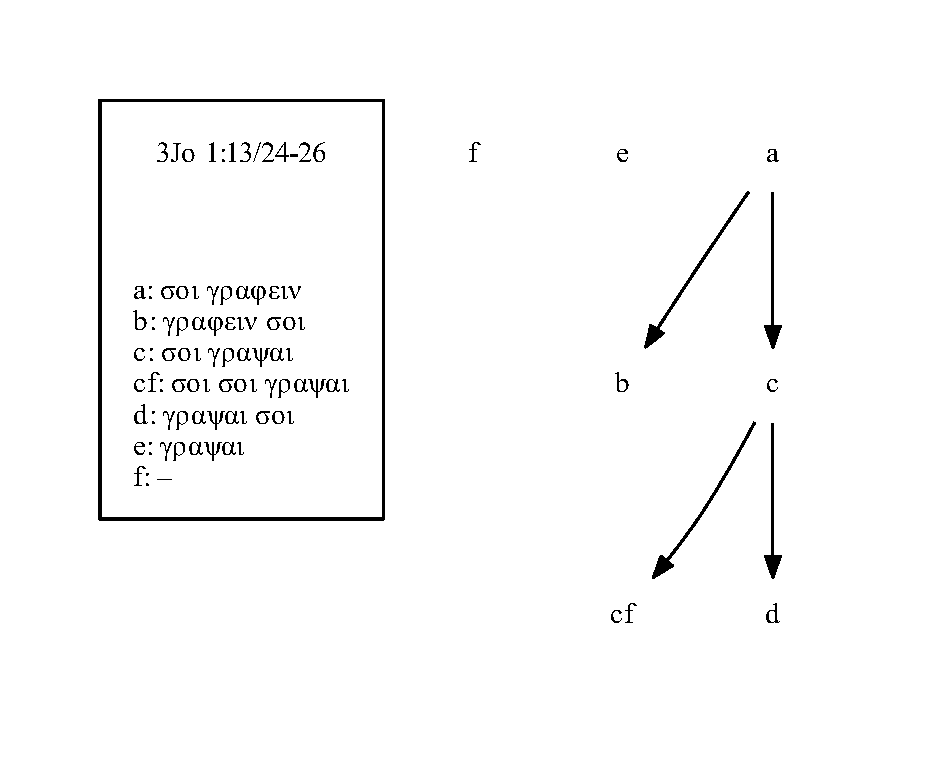
\includegraphics[width=\textwidth]{../img/B25K1V13U24-26-local-stemma-incomplete.pdf}
			\end{column}
			\begin{column}{0.45\textwidth}
				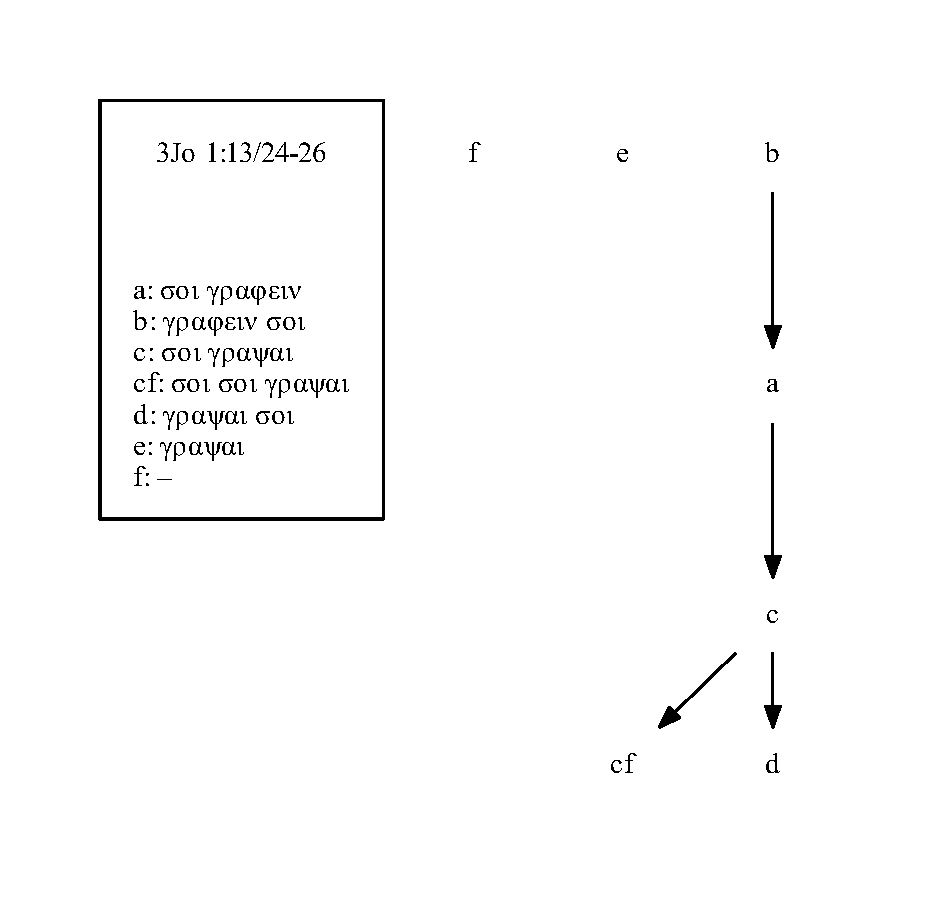
\includegraphics[width=\textwidth]{../img/B25K1V13U24-26-local-stemma-b-initial.pdf}
			\end{column}
		\end{columns}
	\end{frame}
	\begin{frame}
		\begin{center}
			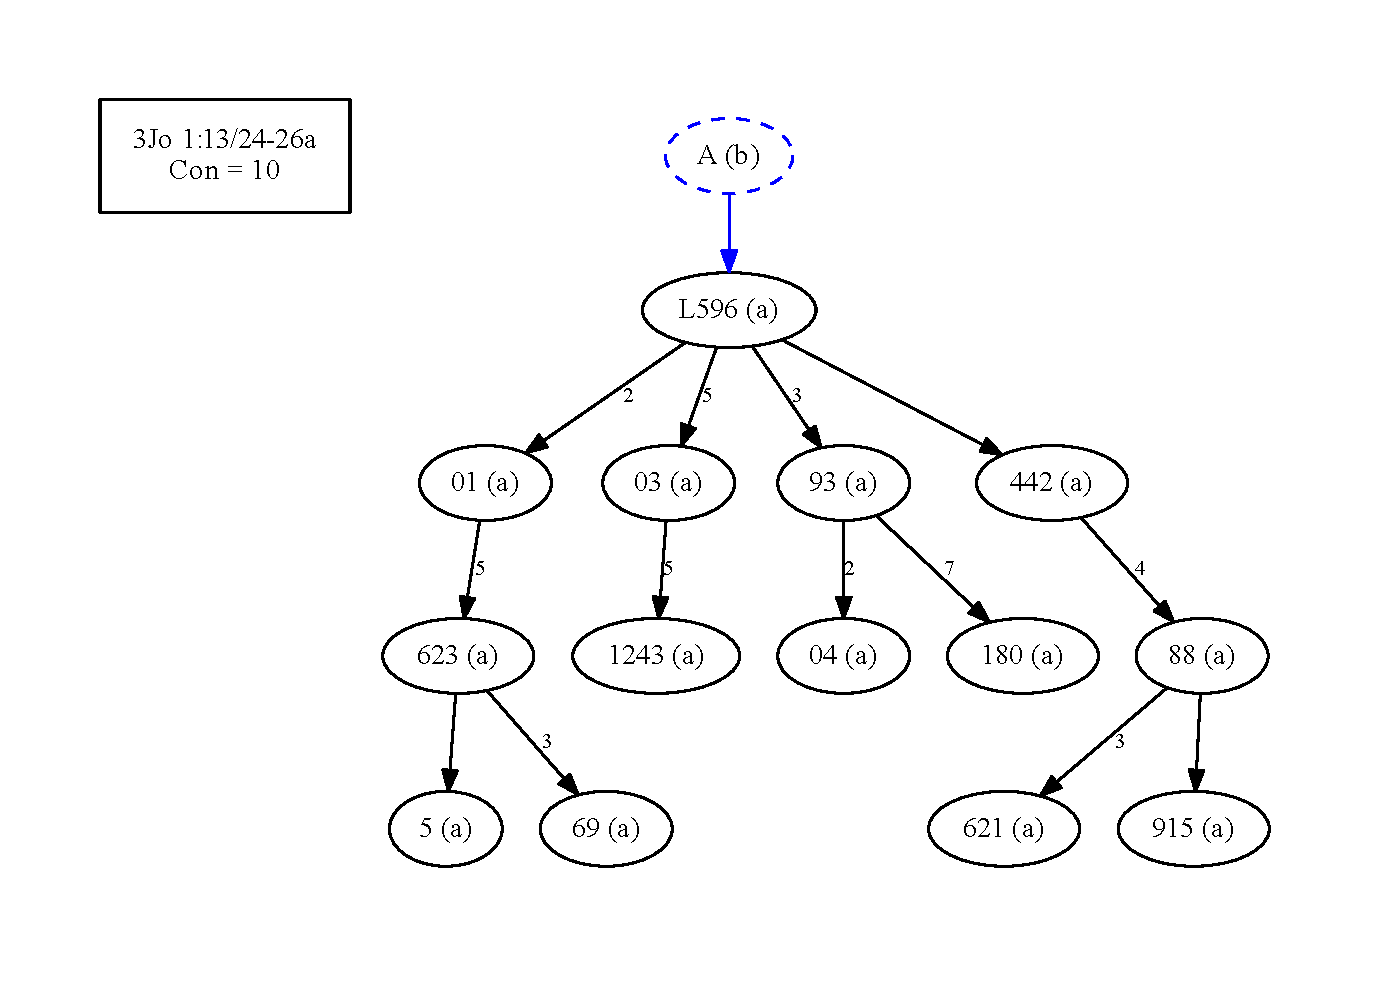
\includegraphics[width=\textwidth]{../img/B25K1V13U24-26Ra-coherence-attestations-b-initial.pdf}
		\end{center}
	\end{frame}
	\begin{frame}
		\begin{columns}
			\begin{column}{0.45\textwidth}
				\begin{itemize}
					\item Or, we can look only at the parts of textual flow where a reading gets changed to find the most likely sources of unexplained readings (\emph{e} and \emph{f})
				\end{itemize}
			\end{column}
			\begin{column}{0.45\textwidth}
				\begin{center}
					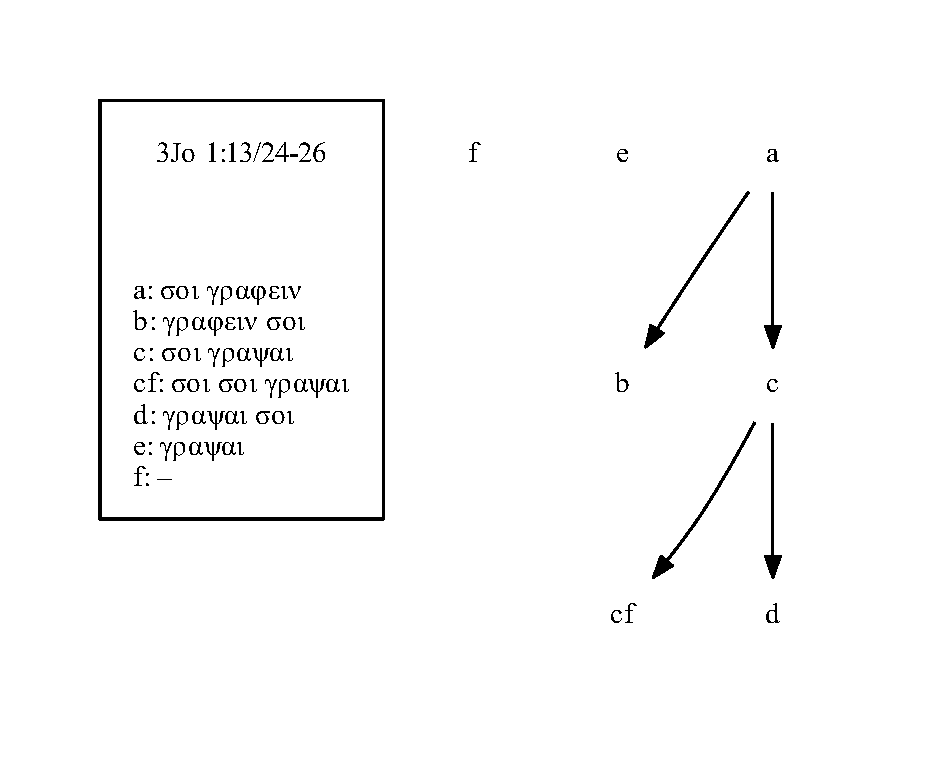
\includegraphics[width=\textwidth]{../img/B25K1V13U24-26-local-stemma-incomplete.pdf}
				\end{center}
			\end{column}
		\end{columns}
	\end{frame}
	\begin{frame}
		\begin{center}
			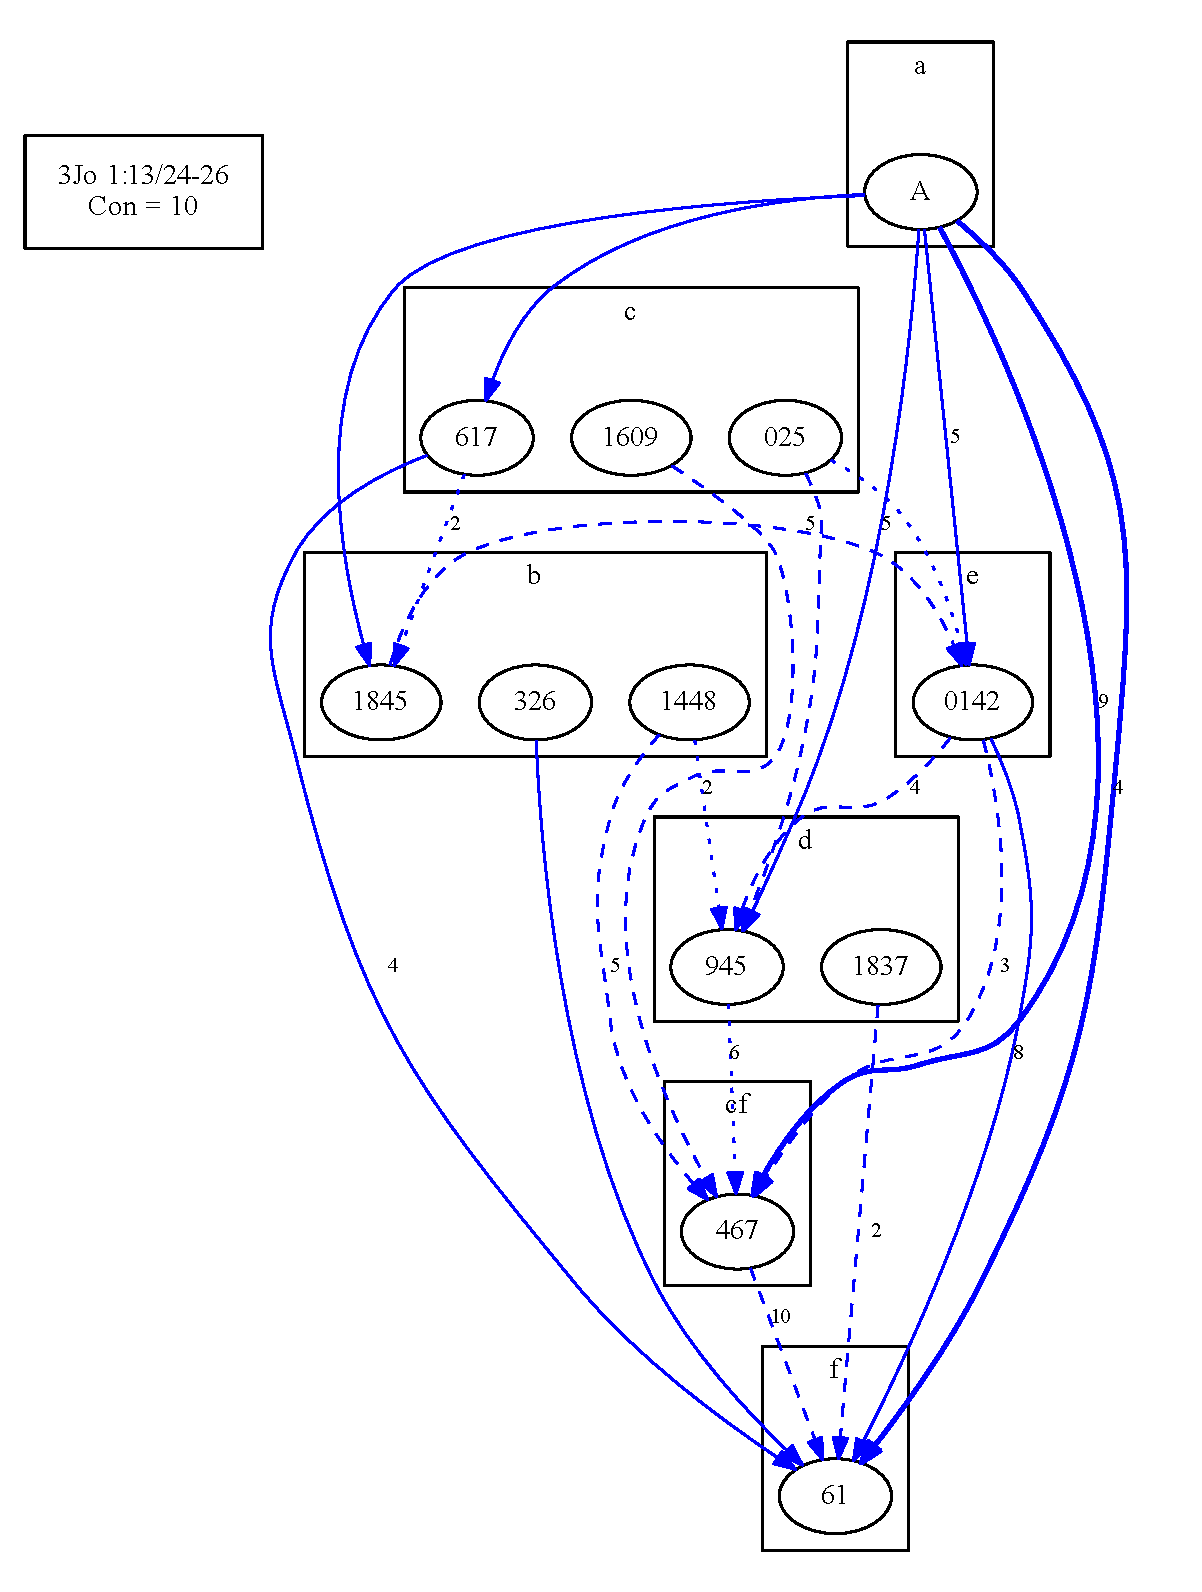
\includegraphics[width=0.5\textwidth]{../img/B25K1V13U24-26-coherence-variants-strengths.pdf}
		\end{center}
	\end{frame}
	\begin{frame}{Textual Flow for a Variant Reading}
		\begin{columns}
			\begin{column}{0.45\textwidth}
				\begin{itemize}
					\item Using this information, we can attempt to explain previous unexplained readings
					\item A necessary step for our ultimate goal of constructing a global stemma
				\end{itemize}
			\end{column}
			\begin{column}{0.45\textwidth}
				\begin{center}
					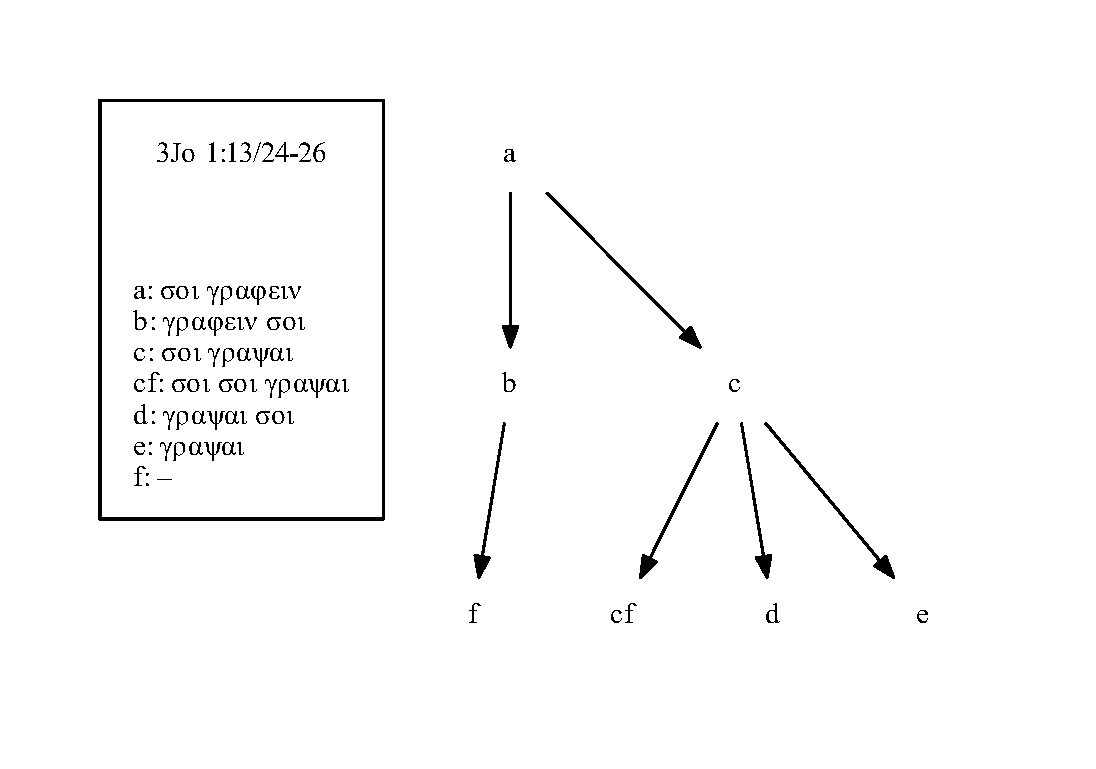
\includegraphics[width=\textwidth]{../img/B25K1V13U24-26-local-stemma-complete.pdf}
				\end{center}
			\end{column}
		\end{columns}
	\end{frame}
	\subsection{\textquote{Explained} Readings}
	\begin{frame}
		\begin{itemize}
			\item We say that one reading \emph{explains} another if
			\begin{itemize}
				\item it is the same reading (explanation by agreement), or
				\item there is an edge in the local stemma from it to the other reading
			\end{itemize}
		\end{itemize}
		\begin{center}
			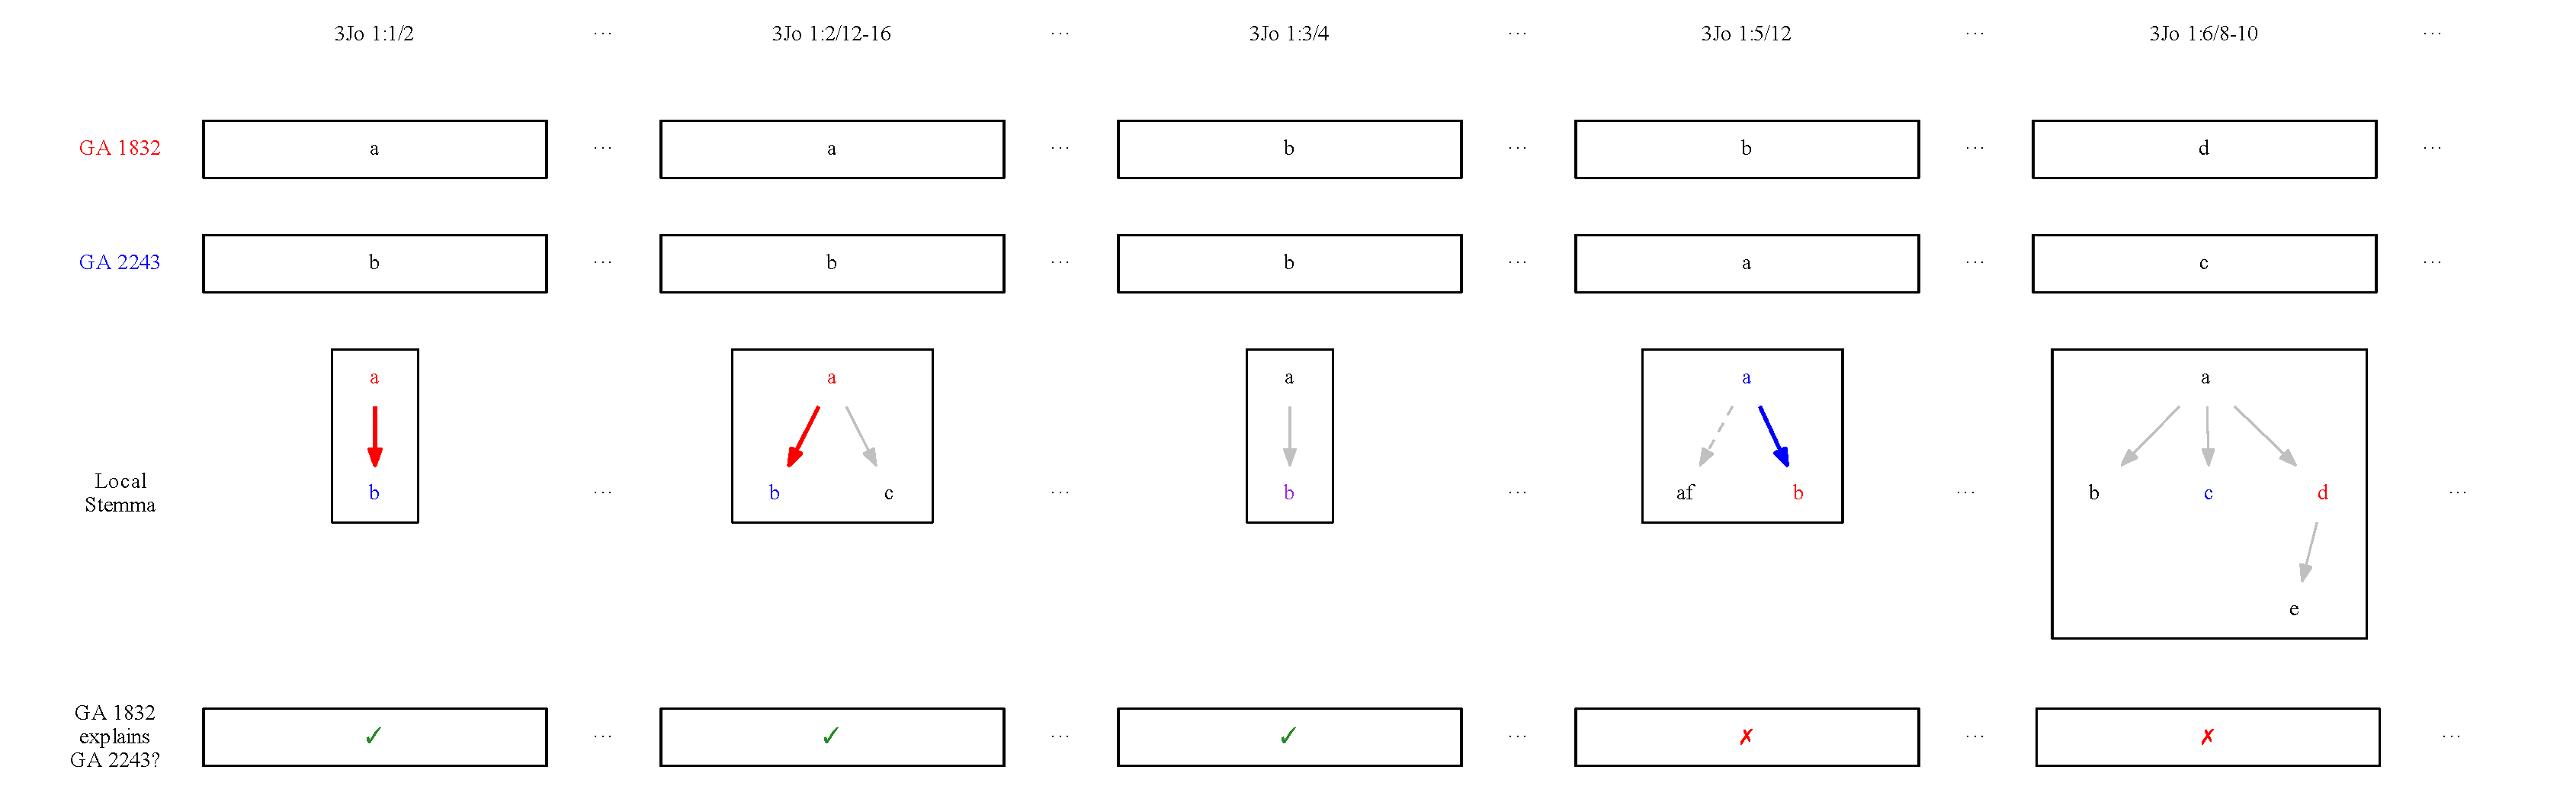
\includegraphics[width=\textwidth]{../img/explained-readings.pdf}
		\end{center}
		\begin{itemize}
			\item Lacunae do not have to be explained, and they cannot explain readings
		\end{itemize}
	\end{frame}
	\begin{frame}
		\begin{columns}
			\begin{column}{0.4\textwidth}
				\centering
				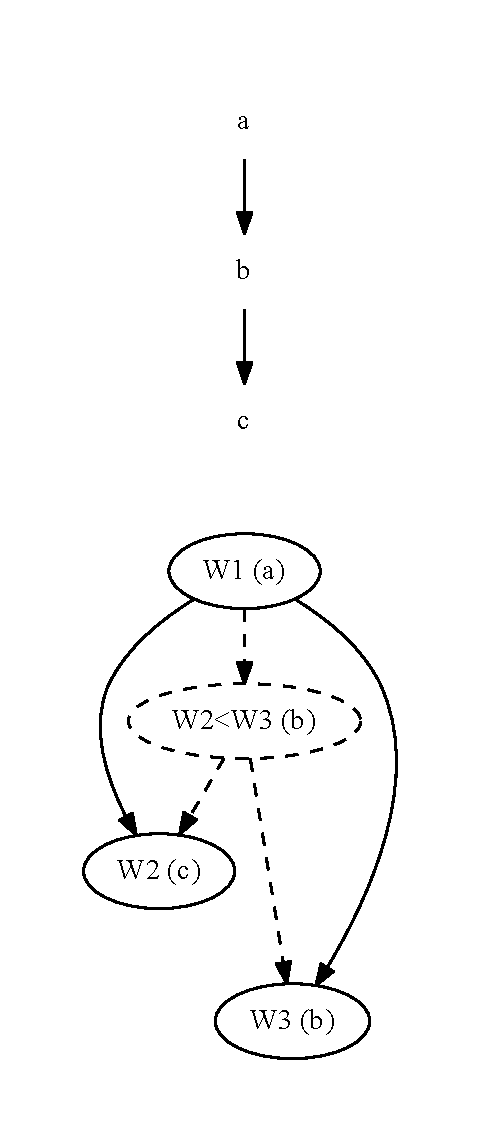
\includegraphics[width=0.75\textwidth]{../img/intermediary-node-example.pdf}
			\end{column}
			\begin{column}{0.55\textwidth}
				\begin{itemize}
					\item Does a reading explain any of its posterior readings transitively (i.e., in the local stemma to the left, does \emph{a} explain \emph{c})?
					\item As originally formulated, \emph{no}: \emph{a} explains \emph{b} and \emph{b} explains \emph{c}, but \emph{a} does not explain \emph{c} (it's too many steps removed)
					\item Later, in the global stemma, \emph{intermediary nodes} may be needed to ensure that all readings are explained
				\end{itemize}
			\end{column}
		\end{columns}
	\end{frame}
	\begin{frame}
		\begin{columns}
			\begin{column}{0.4\textwidth}
				\centering
				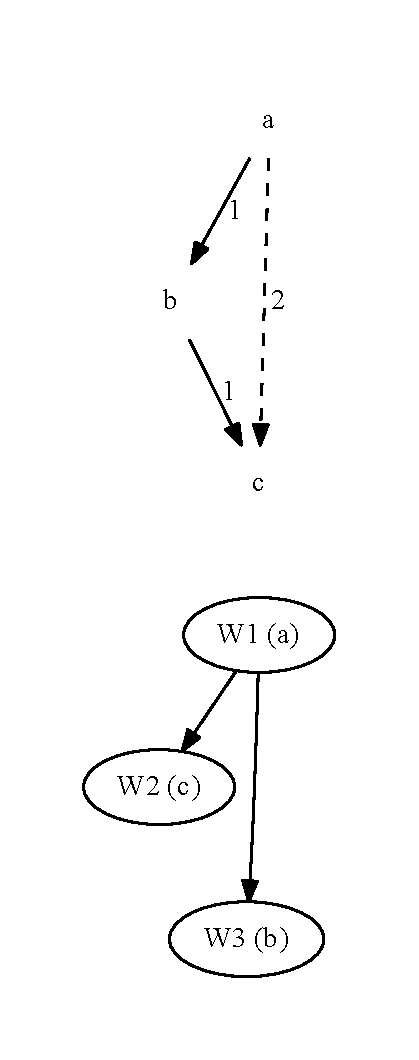
\includegraphics[width=0.75\textwidth]{../img/transitivity-example.pdf}
			\end{column}
			\begin{column}{0.55\textwidth}
				\begin{itemize}
					\item If we instead allow \emph{a} to explain \emph{c}, but at a higher cost (more on this in the substemma slides), then we remove the need for intermediary nodes (although multiple changes in the same variation unit may be implied along an edge in the global stemma)
				\end{itemize}
			\end{column}
		\end{columns}
	\end{frame}
	\begin{frame}{The Substemma(ta) of a Witness}
		\begin{itemize}
			\item The \emph{substemma} of a witness is the portion of the global stemma consisting of the witness and its ancestors in the stemma
			\item Requirement: \emph{every} extant reading in the witness must be explained by a reading in at least one of its ancestors
		\end{itemize}
		\begin{center}
			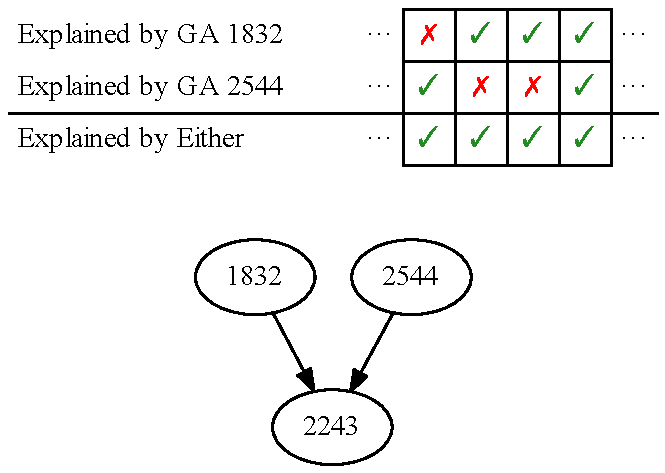
\includegraphics[width=0.75\textwidth]{../img/ga-2243-substemma.pdf}
		\end{center}
	\end{frame}
	\begin{frame}{The Substemma(ta) of a Witness}
		\begin{itemize}
			\item A witness may have multiple valid substemma (i.e., ones that explain all of its readings), but some are better than others
			\item Two of the CBGM's methodological assumptions are important here:
			\begin{enumerate}
				\setcounter{enumi}{2} % manually set the enumerate counter so that the first item is #3
				\item Scribes typically used fewer sources rather than many.
				\item Scribes typically used closely related sources rather than distant ones.
			\end{enumerate}
		\end{itemize}
		\begin{center}
			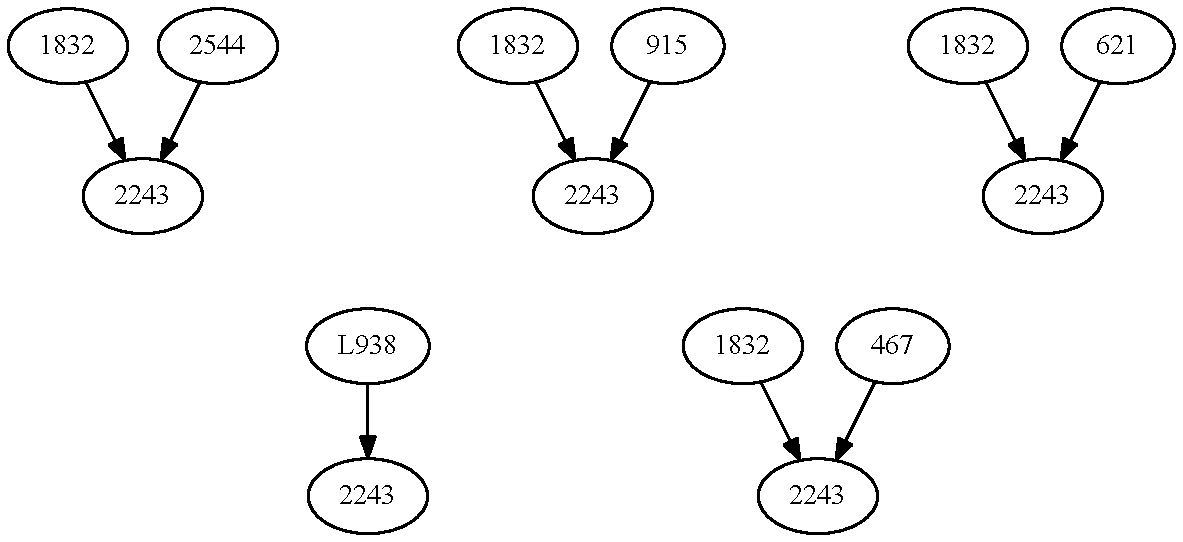
\includegraphics[width=0.75\textwidth]{../img/substemmata.pdf}
		\end{center}
	\end{frame}
	\begin{frame}{The Substemma(ta) of a Witness}
		\begin{itemize}
			\item Based on assumption 3, we should prefer substemmata with fewer ancestors (``parsimony'')
			\item Based on assumption 4, we should prefer substemmata with ancestors that agree as often as possible with the witness
			\item A balancing act: the substemma \{L938\} is more parsimonious, but may not explain as many readings by agreement
		\end{itemize}
		\begin{center}
			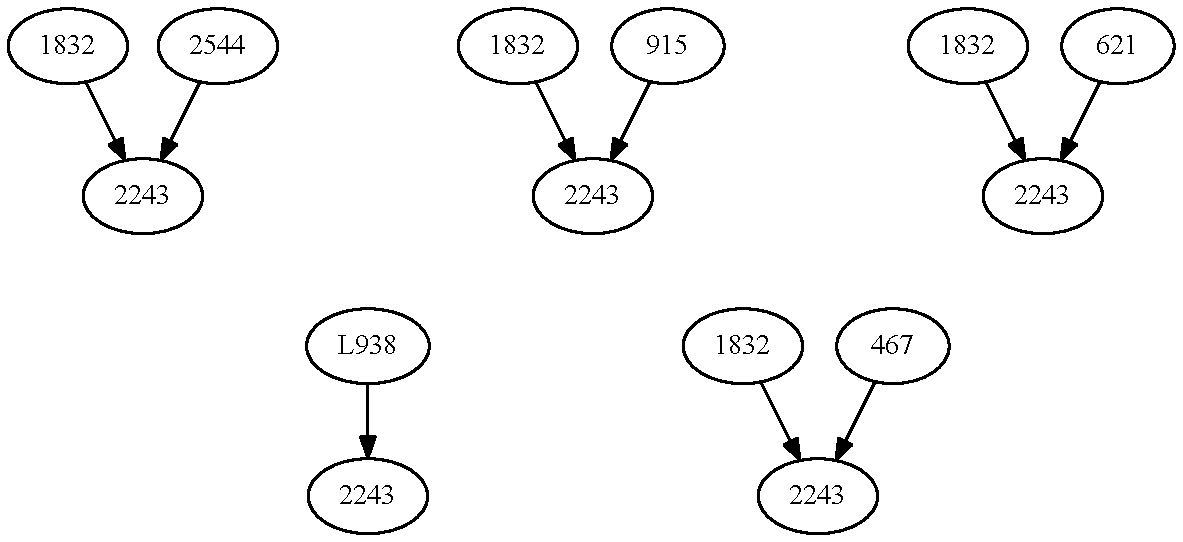
\includegraphics[width=0.75\textwidth]{../img/substemmata.pdf}
		\end{center}
	\end{frame}
	\begin{frame}{The Substemma(ta) of a Witness}
		\begin{itemize}
			\item A simple cost function for each ancestor is ``the number of variation units where the ancestor explains the witness by descent and not agreement''
		\end{itemize}
		\begin{center}
			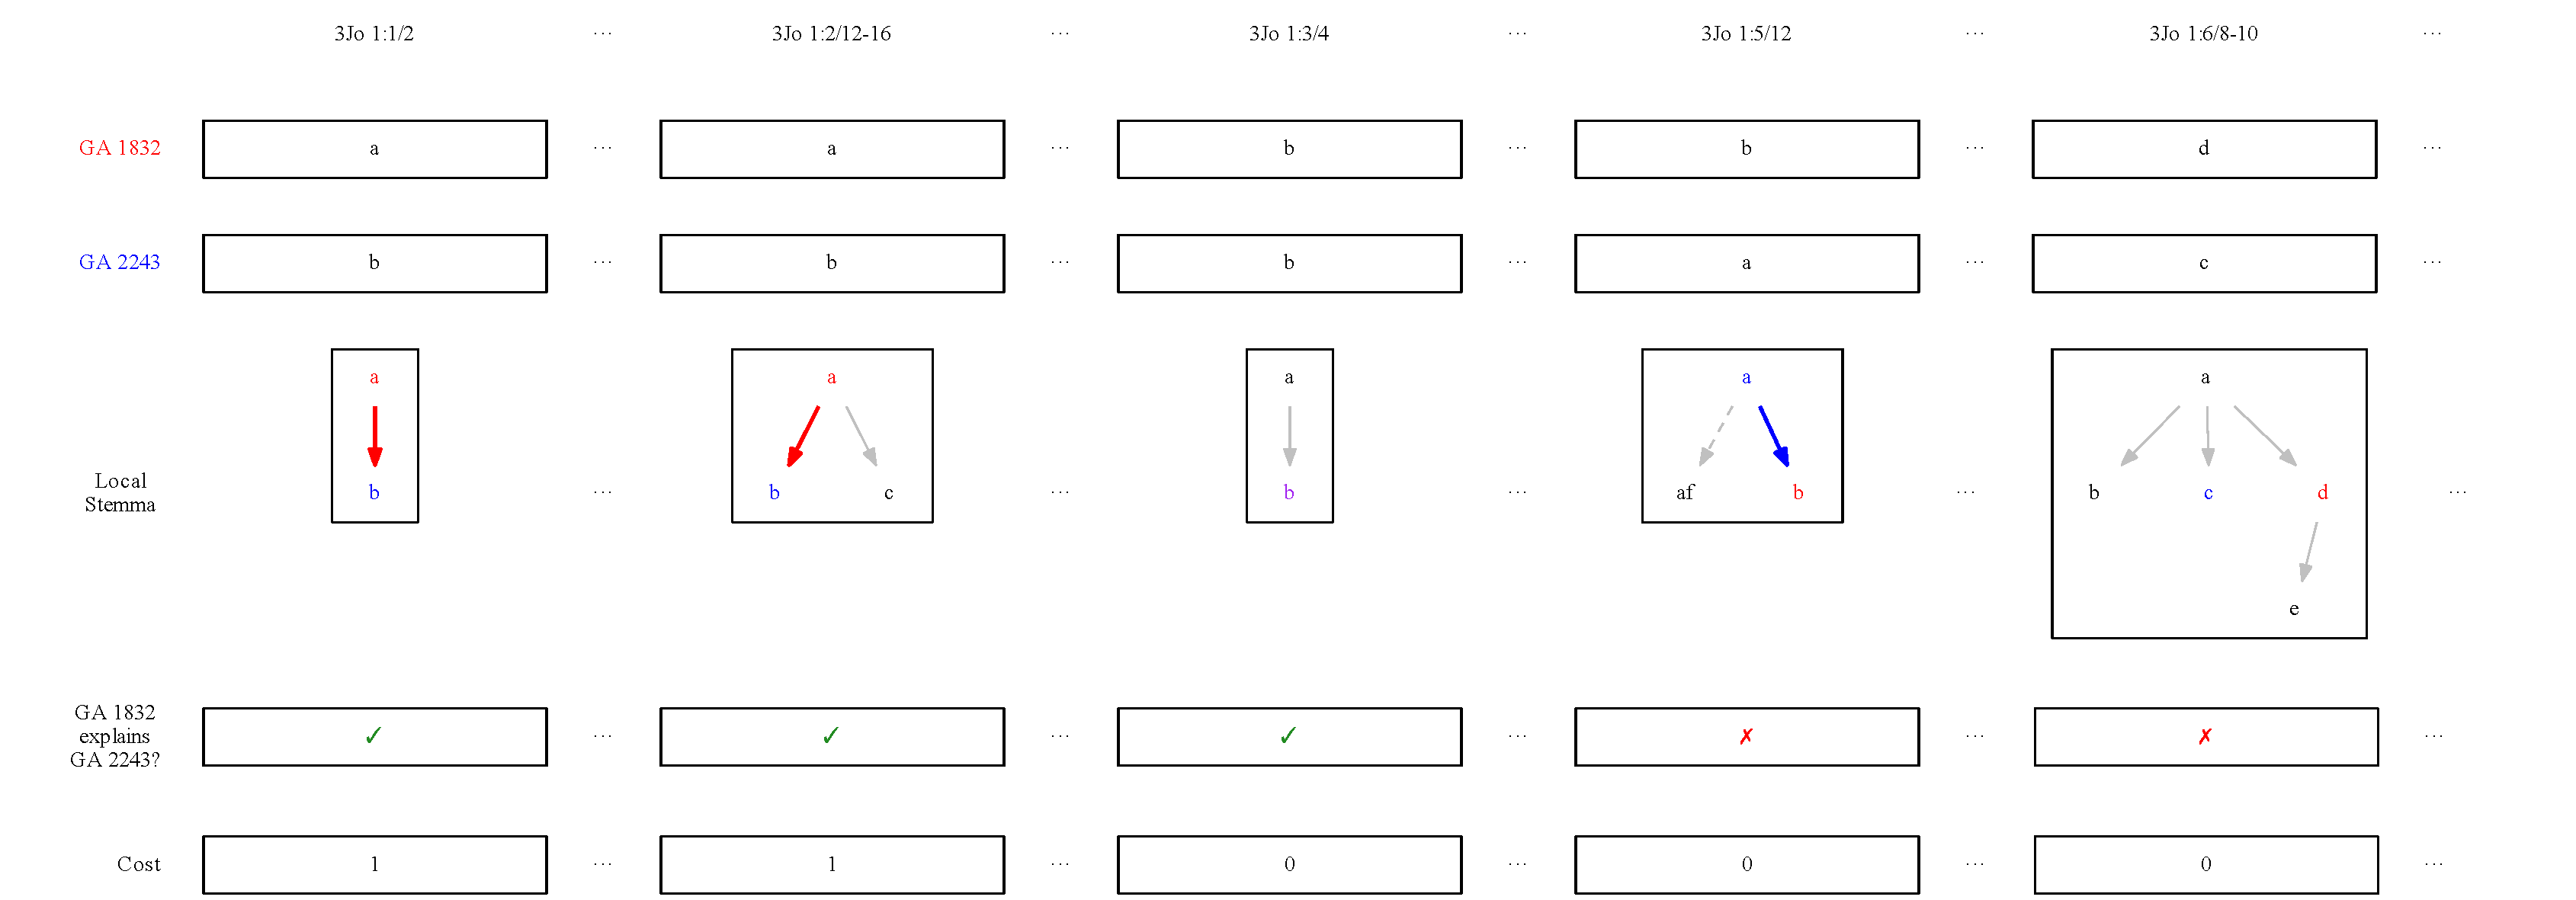
\includegraphics[width=\textwidth]{../img/explained-readings-costs.pdf}
		\end{center}
	\end{frame}
	\begin{frame}{The Substemma(ta) of a Witness}
		\begin{columns}
			\begin{column}{0.45\textwidth}
				\begin{itemize}
					\item If we allow a reading to explain any reading posterior to it, then a better cost per variation unit is the length of the path from the prior reading to the posterior one.
				\end{itemize}
			\end{column}
			\begin{column}{0.45\textwidth}
				\begin{center}
					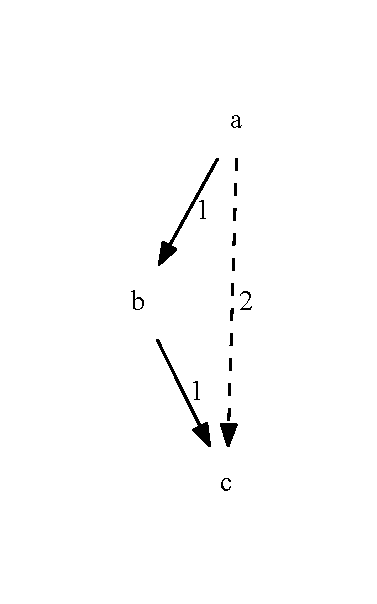
\includegraphics[width=0.75\textwidth]{../img/transitivity-cost.pdf}
				\end{center}
			\end{column}
		\end{columns}
	\end{frame}
	\begin{frame}{Finding a (Good) Substemma}
		\begin{itemize}
			\item Also called \emph{substemma optimization}
			\item For $n$ potential ancestors, a \emph{weighted set cover} problem with $n$ sets (and $2^n - 1$ combinations to check!)
		\end{itemize}
		\begin{center}
			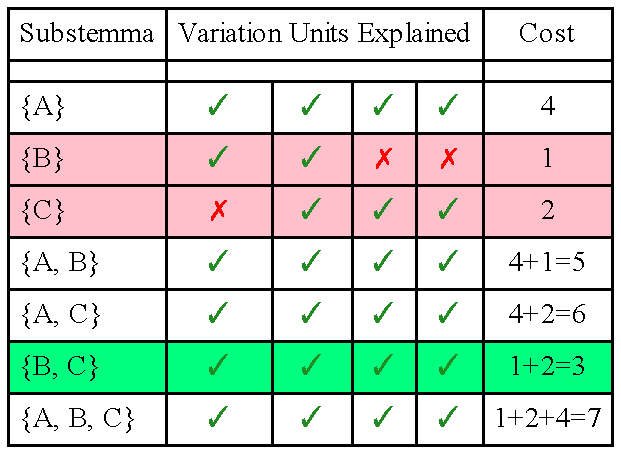
\includegraphics[width=0.75\textwidth]{../img/weighted-set-cover.pdf}
		\end{center}
	\end{frame}
	\begin{frame}{Finding a (Good) Substemma}
		\begin{columns}
			\begin{column}{0.4\textwidth}
				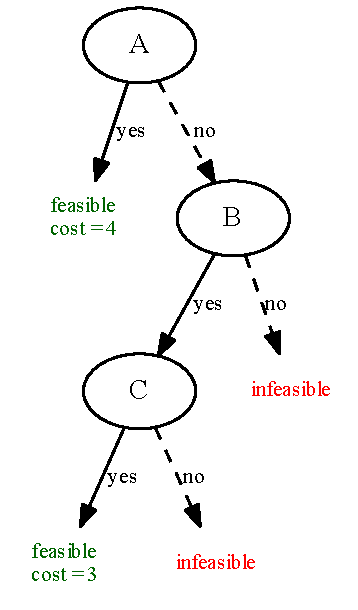
\includegraphics[width=\textwidth]{../img/branch-and-bound-example.pdf}
			\end{column}
			\begin{column}{0.55\textwidth}
				\begin{itemize}
					\item If a witness has many potential ancestors, then checking all $2^n - 1$ possible substemmata by brute force is prohibitive
					\item The \emph{branch-and-bound} heuristic (pictured left) finds all minimum-cost substemmata quickly in practice
					\item Easily adapted to find all substemmata within a given cost
				\end{itemize}
			\end{column}
		\end{columns}
	\end{frame}
	\begin{frame}{The Global Stemma}
		\begin{columns}
			\begin{column}{0.45\textwidth}
				\begin{itemize}
					\item Just as the local stemma relates readings, the \emph{global stemma} relates witnesses
					\item Combination of all substemmata into a single graph
				\end{itemize}
			\end{column}
			\begin{column}{0.45\textwidth}
				\begin{center}
					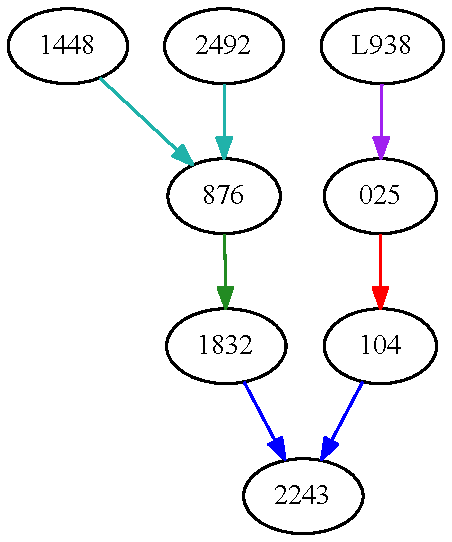
\includegraphics[width=\textwidth]{../img/partial-global-stemma.pdf}
				\end{center}
			\end{column}
		\end{columns}
	\end{frame}
	\begin{frame}{The Global Stemma}
		\begin{columns}
			\begin{column}{0.45\textwidth}
				\begin{itemize}
					\item But \emph{every reading in every local stemma} except the initial one must be explained by another reading
					\item Otherwise…
				\end{itemize}
			\end{column}
			\begin{column}{0.45\textwidth}
				\begin{center}
					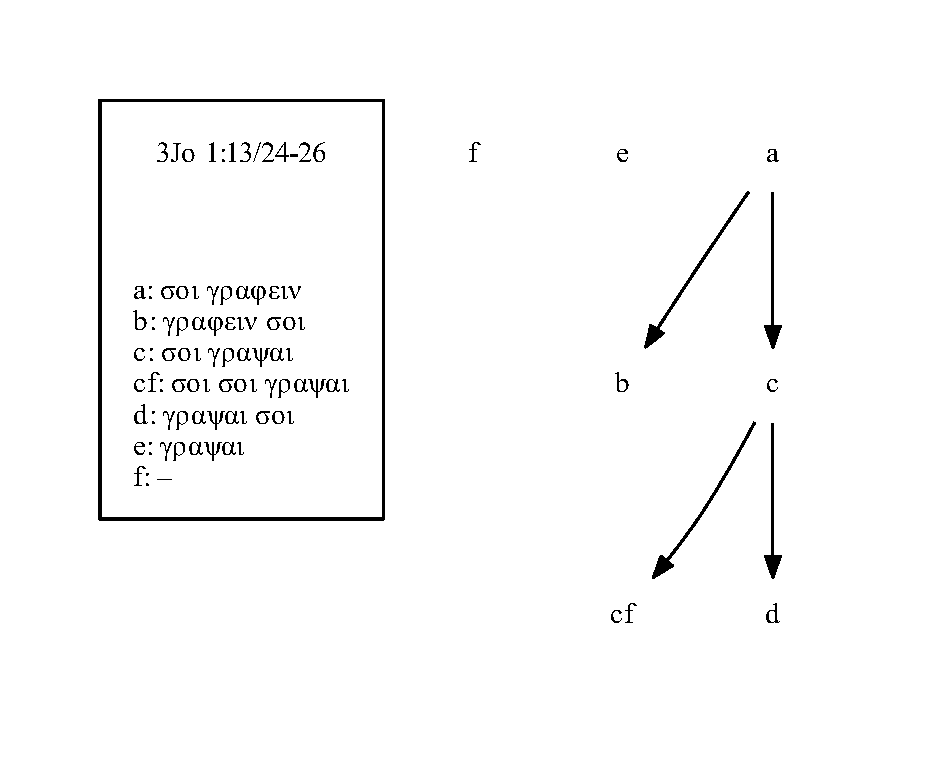
\includegraphics[width=0.875\textwidth]{../img/B25K1V13U24-26-local-stemma-incomplete.pdf}
				\end{center}	
			\end{column}
		\end{columns}
		\begin{center}
			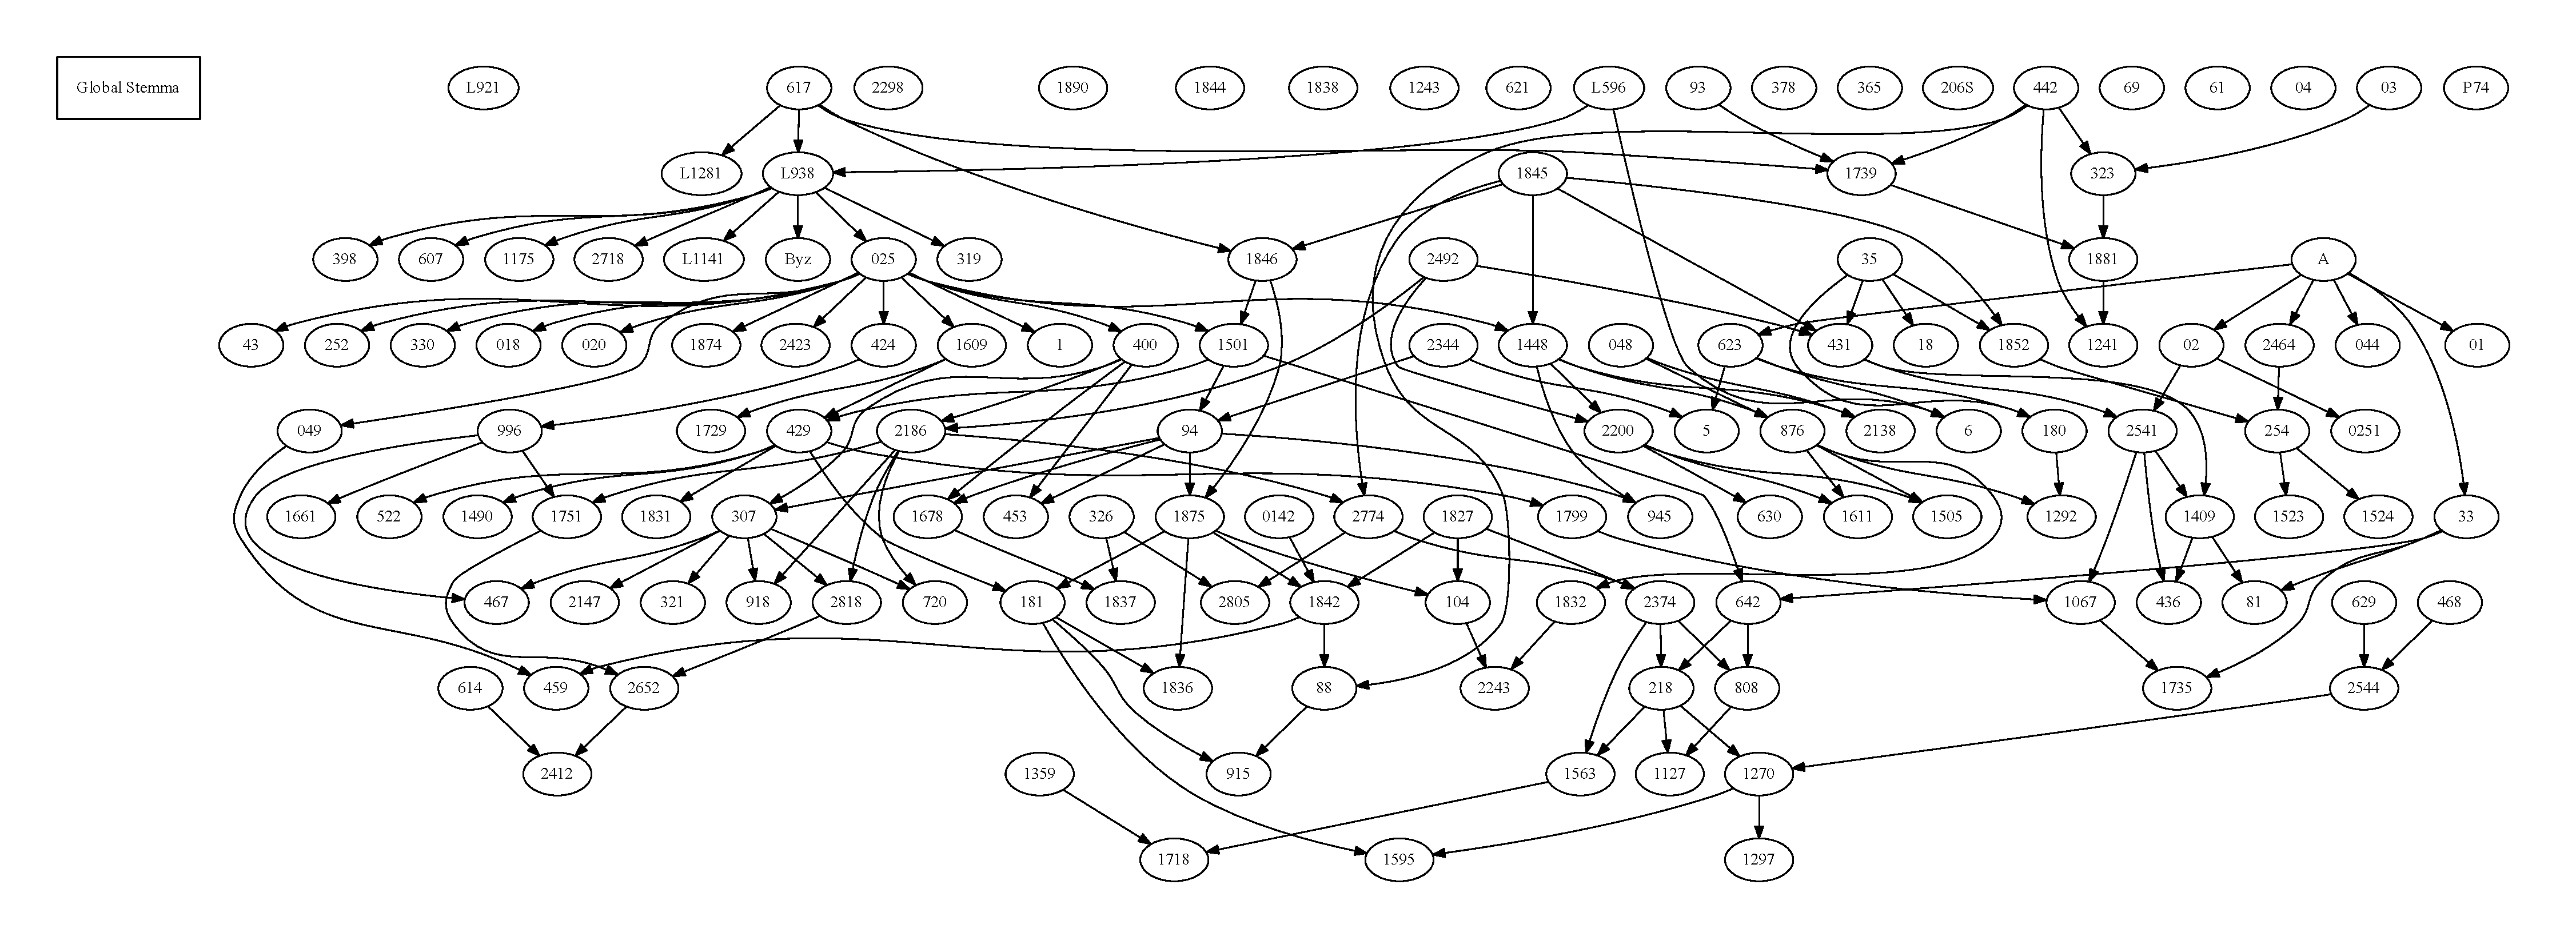
\includegraphics[width=\textwidth]{../img/global-stemma-incomplete.pdf}
		\end{center}	
	\end{frame}
	\begin{frame}{The Global Stemma}
		\begin{columns}
			\begin{column}{0.45\textwidth}
				\begin{itemize}
					\item If we ``complete'' every local stemma (and ignore or manually account for super fragmentary witnesses) ...
				\end{itemize}
			\end{column}
			\begin{column}{0.45\textwidth}
				\begin{center}
					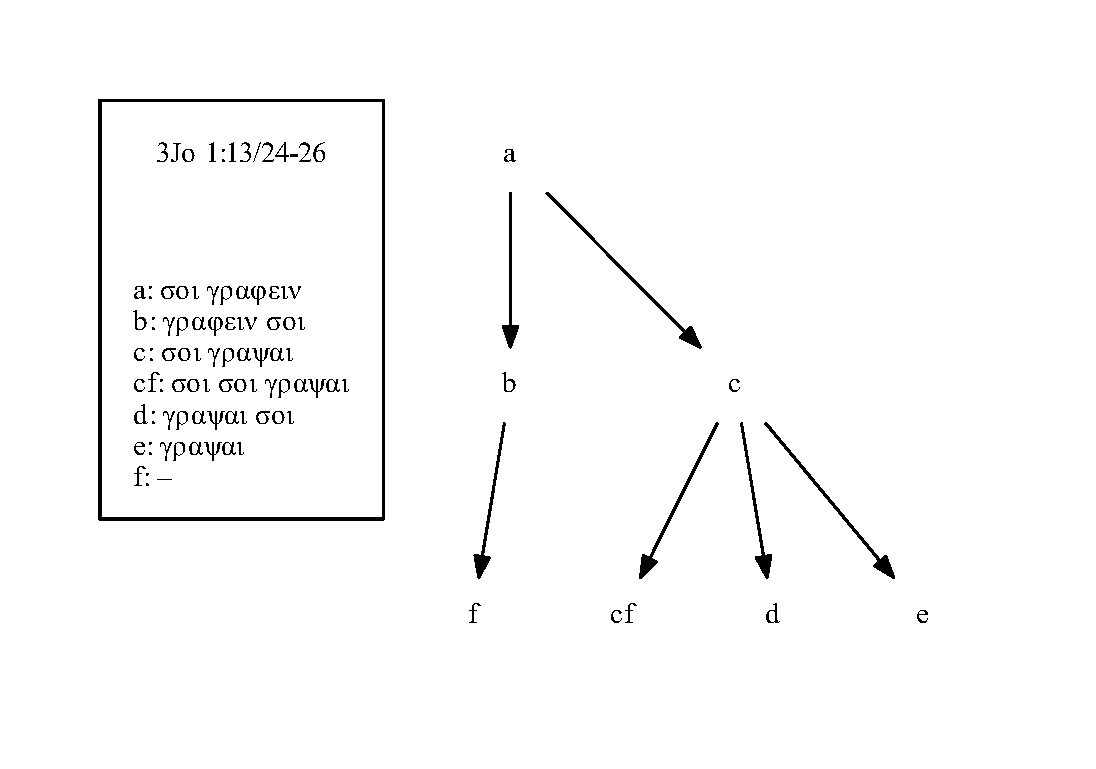
\includegraphics[width=\textwidth]{../img/B25K1V13U24-26-local-stemma-complete.pdf}
				\end{center}	
			\end{column}
		\end{columns}
		\begin{center}
			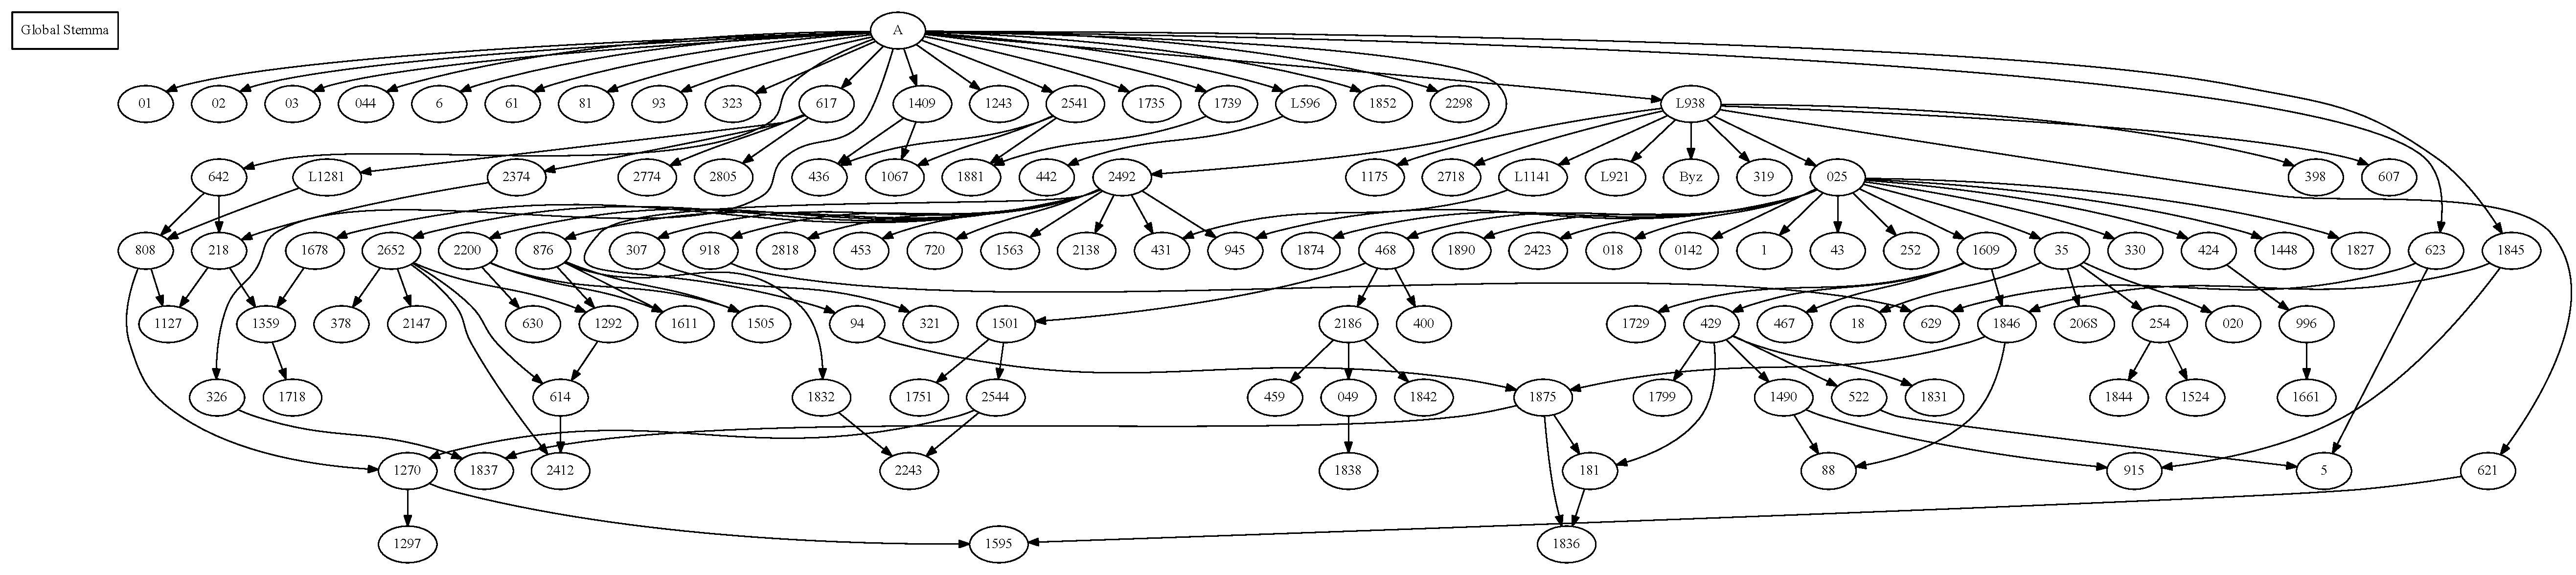
\includegraphics[width=\textwidth]{../img/global-stemma-complete.pdf}
		\end{center}	
	\end{frame}
	\begin{frame}{The Global Stemma}
		\begin{itemize}
			\item How is this different than a textual flow diagram?
			\begin{itemize}
				\item A witness can have more than one ancestor
				\item All readings in a witness must be explained by readings in its ancestor(s)
				\item More computationally intensive, so takes a bit longer to produce
			\end{itemize}
		\end{itemize}
		\begin{center}
			\href{../img/global-stemma-complete-reoriented.pdf}{*Field trip*}
		\end{center}
	\end{frame}
	\begin{frame}{Criticisms and Idiosyncrasies}
		\begin{itemize}
			\item Biggest idiosyncrasy: \emph{no reconstruction of hypothetical ancestors} (because contamination is assumed to make this impossible)
			\begin{itemize}
				\item (Personal opinion: this assumption is made for practical rather than theoretical reasons)
				\item Texts of extant witnesses = bad representatives of ancestors of other extant texts
				\item CBGM may see ``contamination'' where there's just a gap in the textual tradition
				\item Enough of the tradition is lost to make this a problem
			\end{itemize}
			\item Can the global stemma be understood as a history of the text?
		\end{itemize}
	\end{frame}
	\begin{frame}{Criticisms and Idiosyncrasies}
		\begin{itemize}
			\item Recommended reading:
			\begin{itemize}
				\item \cite{Jongkind14}
				\item The special feature articles in \emph{TC} 20 (2015)
				\item \cite{Gurry18}
				\item \cite{Carlson20} (but see \href{http://ntvmr.uni-muenster.de/en_US/intfblog/-/blogs/remarks-on-carlson-a-bias-at-the-heart-of-the-cbgm-guest-post-by-gerd-mink-}{Mink's response})
			\end{itemize}
		\end{itemize}
	\end{frame}
%	\section{Hort and the Stemmatic Model}
%	\begin{frame}
%		\begin{columns}
%			\begin{column}{0.35\textwidth}
%				\begin{center}
%					\only<1>{
%						\includegraphics[width=\textwidth]{../img/westcott-hort-original.png}\\
%						\footnotesize Source: Wikimedia Commons\\
%						\phantom{(with adaptations)}
%					}
%					\only<2>{
%						\includegraphics[width=0.675\textwidth]{../img/hort-westcott-bookends.pdf}\\
%						\footnotesize Source: Wikimedia Commons\\
%						(with adaptations)
%					}
%				\end{center}
%				\vspace{0.5\baselineskip}
%				\begin{itemize}
%					\item Red, dotted = \emph{intrinsic probability}
%					\item Green, dashed = \emph{transcriptional probability}
%					\item Blue, solid = \emph{genealogical evidence}
%				\end{itemize}
%			\end{column}
%			\begin{column}{0.65\textwidth}
%				\includegraphics[width=\textwidth]{../img/stemma-evidence-overlay.pdf}
%			\end{column}
%		\end{columns}
%	\end{frame}
%	\section{Intrinsic Probability}
%	\begin{frame}
%		\begin{itemize}
%			\item Similar to the rating system used in the UBS Commentary
%		\end{itemize}
%		\vspace{0.5\baselineskip}
%		\begin{tabular}{p{0.25\textwidth} p{0.7\textwidth}}
%			\emph{Rating} & \emph{Description}\\
%			\hline
%			\Rdg{a} \RelativeRating{A} \Rdg{b} & Reading \Rdg{a} is \emph{absolutely more likely} than reading \Rdg{b}.\\
%			\Rdg{a} \RelativeRating{B} \Rdg{b} & Reading \Rdg{a} is \emph{highly more likely} than reading \Rdg{b}.\\
%			\Rdg{a} \RelativeRating{C} \Rdg{b} & Reading \Rdg{a} is \emph{more likely} than reading \Rdg{b}.\\
%			\Rdg{a} \RelativeRating{D} \Rdg{b} & Reading \Rdg{a} is \emph{slightly more likely} than reading \Rdg{b}.\\
%			\Rdg{a} \EqualRating{} \Rdg{b} & Readings \Rdg{a} and \Rdg{b} have equal probability.
%		\end{tabular}
%		\vspace{0.5\baselineskip}
%		\begin{columns}[T]
%			\begin{column}{0.55\textwidth}
%				\begin{itemize}
%					\item Odds ratios between one reading and the next most likely one
%					\item e.g., \Rdg{b} \RelativeRating{D} \Rdg{c} \RelativeRating{A} \Rdg{a} \EqualRating{} \Rdg{d} (right)
%					\item Example values: $A = 19$, $B = 4$, $C = 1.5$, and $D = 1.1$
%				\end{itemize}
%			\end{column}
%			\begin{column}{0.4\textwidth}
%				\includegraphics[width=\textwidth]{../img/intrinsic-probabilities-bar-chart.pdf}
%			\end{column}
%		\end{columns}
%	\end{frame}
%	\section{Transcriptional Probability}
%	\begin{frame}
%		\begin{itemize}
%			\item A system of labels whose relative frequencies will be evaluated as part of the model
%		\end{itemize}
%		\begin{center}
%			\begin{tabular}{p{0.25\textwidth} p{0.7\textwidth}}
%					\emph{Tag} & \emph{Description}\\
%					\hline
%					\Clarification{} & Clarification in terms of grammar, style, or theology\\
%					\AuralConfusion{} & Confusion of similar sounds (\textgreek{ι}/\textgreek{ει}/\textgreek{η}/\textgreek{οι}/\textgreek{υ}, \textgreek{αι}/\textgreek{ε}, \textgreek{ο}/\textgreek{ω}, \textgreek{β}/consonantal \textgreek{υ}, \textgreek{π}/\textgreek{φ}, \textgreek{κτλ}.)\\
%					\LinguisticConfusion{} & Changes due to unfamiliarity with Greek grammar or changes to its rules over time\\
%					\VisualError{} & Visual confusion of similar letters, skips and duplications of letters or words\\
%					\Harmonization{} & Harmonization to parallel passage or near context\\
%					\Byzantine{} & Assimilation to the dominant Byzantine text
%			\end{tabular}
%		\end{center}
%		\begin{itemize}
%			\item This allows us to model (and measure) different classes of scribal habits and a common type of mixture
%		\end{itemize}
%	\end{frame}
%	\begin{frame}
%		\begin{itemize}
%			\item We can tag transitions between variant readings in a given unit according to their potential causes
%			\item A stemma's probability is calculated along its branches in terms of transcriptional rates using \emph{Markov chains} (see below)
%		\end{itemize}
%		\begin{columns}[T]
%			\begin{column}{0.5\textwidth}
%				\footnotesize
%				Eph 5:22\\
%				\vspace{\baselineskip}
%				\Rdg{a}: \textgreek{τοις ιδιοις ανδρασιν υποτασσεσθωσαν}\\
%				\Rdg{b}: \textgreek{υποτασσεσθωσαν τοις ιδιοις ανδρασιν}\\
%				\Rdg{c}: \textgreek{τοις ιδιοις ανδρασιν υποτασσεσθε}\\
%				\Rdg{d}: \textgreek{υποτασσεσθε τοις ιδιοις ανδρασιν}\\
%				\Rdg{e}: \textgreek{τοις ιδιοις ανδρασιν υποτασσομεναι}\\
%				\Rdg{f}: \textgreek{τοις ιδιοις ανδρασιν} 
%			\end{column}
%			\begin{column}{0.5\textwidth}
%				\includegraphics[scale=0.75]{../img/K5V22U6-12-transcriptional-probabilities.pdf}
%			\end{column}
%		\end{columns}
%		\begin{itemize}
%			\item Looks and functions like a local stemma, but is less constrained
%		\end{itemize}
%	\end{frame}
%	\section{Genealogical Evidence}
%	\begin{frame}
%		\begin{itemize}
%			\item Given a hypothesis $\mathcal{H}$ (i.e., a stemma with its parameters describing intrinsic probabilities, transcriptional probabilities, etc.) about how our collation data $\mathcal{D}$ arose, we can calculate its \emph{explanatory power} or \emph{likelihood} $\Pr(\mathcal{D} \mid \mathcal{H})$ using phylogenetic algorithms
%			\item The \emph{posterior probability} $\Pr(\mathcal{H} \mid \mathcal{D})$ tells us how certain we can be about $\mathcal{H}$; we can estimate it by cleverly sampling different stemmata and combinations of parameters
%		\end{itemize}
%		\vspace{3\baselineskip}
%		\begin{equation*}
%			{\color{blue}\overbrace{\color{black}\Pr(\mathcal{H} \mid \mathcal{D})}^{\text{Posterior}}}
%			= \frac{
%			{\color{red}\overbrace{\color{black}\Pr(\mathcal{D} \mid \mathcal{H})}^{\text{Likelihood}}}
%			{\color{green!50!black}\overbrace{\color{black}\Pr(\mathcal{H})}^{\text{Prior}}}
%			}{
%			{\color{orange}\underbrace{{\color{black}\Pr(\mathcal{D})}}_{\text{Probability of Data}}}
%			}
%		\end{equation*}
%		\vspace{3.75\baselineskip}
%	\end{frame}
%	\section{Impact}
%	\begin{frame}
%		\only<1>{
%			\begin{center}
%				\includegraphics[scale=1]{../img/paul-comic.png}\\
%				\footnotesize Source: Rembrandt van Rijn, \emph{The Apostle Paul} (Wikimedia Commons)\\
%			\end{center}
%		}
%		\only<2->{
%			\emph{Much in many ways!}
%			\begin{itemize}
%				\item<3-> A clean separation of concerns between different types of evidence
%				\item<4-> Accommodation and resolution of tension between intrinsic and transcriptional evidence
%				\item<5-> Built-in estimation of scribal habits
%				\item<6-> Support for witness dates
%				\item<7-> Inclusion of (sufficiently extant) versional and patristic sources
%				\item<8-> A measure of (un)certainty about stemma branches, scribal habits, initial readings
%				\item<9-> A set of candidate stemmata that can be reconciled to address contamination in a local-genealogical way
%			\end{itemize}
%		}
%	\end{frame}
%	\section{Demonstration}
%	\subsection{1 Peter}
%	\begin{frame}
%		\begin{center}
%			\includegraphics[width=\textwidth]{../img/ubs_1_peter_local_densitree.pdf}\\
%			Posterior distribution of stemmata for subset of UBS 1 Peter data at UBS variation units (64 witnesses, 36 variation units, 20,000,000 iterations) with local clock model\\
%		\end{center}
%	\end{frame}
%	\subsection{Revelation}
%	\begin{frame}
%		\begin{center}
%			\includegraphics[width=0.6667\textwidth]{../img/ubs_revelation_local_densitree.pdf}\\
%			Posterior distribution of stemmata for subset of UBS Revelation data at UBS variation units (33 witnesses, 70 variation units, 20,000,000 iterations) with local clock model\\
%		\end{center}
%	\end{frame}
%	\begin{frame}
%		\begin{center}
%			\includegraphics[width=\textwidth]{../img/ubs_revelation_local_max_clade_credibility_tree.pdf}\\
%			Maximum clade credibility tree for subset of UBS Revelation data at UBS variation units (33 witnesses, 70 variation units, 20,000,000 iterations) with local clock model\\
%		\end{center}
%	\end{frame}
%	\subsection{Mark}
%	\begin{frame}
%		\begin{center}
%			\includegraphics[width=\textwidth]{../img/ecm_mark_local_densitree.pdf}\\
%			Posterior distribution of stemmata for ECM Mark data at UBS variation units (167 witnesses, 148 variation units, 20,000,000 iterations) with local clock model\\
%		\end{center}
%	\end{frame}
%	\begin{frame}
%		\begin{center}
%			\includegraphics[width=\textwidth]{../img/ecm_mark_local_max_clade_credibility_tree_a_text.png}\\
%			Subset of maximum clade credibility tree for ECM Mark data at UBS variation units (167 witnesses, 148 variation units, 20,000,000 iterations) with local clock model\\
%		\end{center}
%	\end{frame}
%	\begin{frame}
%		\begin{center}
%			\includegraphics[width=\textwidth]{../img/ecm_mark_local_max_clade_credibility_tree_family_041.png}\\
%			Subset of maximum clade credibility tree for ECM Mark data at UBS variation units (167 witnesses, 148 variation units, 20,000,000 iterations) with local clock model\\
%		\end{center}
%	\end{frame}
%	\begin{frame}
%		\begin{center}
%			\includegraphics[width=\textwidth]{../img/ecm_mark_local_max_clade_credibility_tree_family_1216.png}\\
%			Subset of maximum clade credibility tree for ECM Mark data at UBS variation units (167 witnesses, 148 variation units, 20,000,000 iterations) with local clock model\\
%		\end{center}
%	\end{frame}
%	\begin{frame}
%		\begin{center}
%			\includegraphics[width=\textwidth]{../img/ecm_mark_local_max_clade_credibility_tree_caesarean.png}\\
%			Subset of maximum clade credibility tree for ECM Mark data at UBS variation units (167 witnesses, 148 variation units, 20,000,000 iterations) with local clock model\\
%		\end{center}
%	\end{frame}
%	\begin{frame}
%		\begin{center}
%			\includegraphics[width=\textwidth]{../img/ecm_mark_local_rates.pdf}\\
%			Transcriptional rate posteriors for ECM Mark data at UBS variation units (167 witnesses, 148 variation units, 20,000,000 iterations) with local clock model\\
%		\end{center}
%	\end{frame}
%		\subsection{Ephesians}
%	\begin{frame}
%		\begin{center}
%			\includegraphics[width=\textwidth]{../img/ubs_ephesians_local_densitree.pdf}\\
%			Posterior distribution of stemmata for subset of UBS Ephesians data at UBS variation units (36 witnesses, 42 variation units, 20,000,000 iterations) with local clock model\\
%		\end{center}
%	\end{frame}
%	\begin{frame}
%		\begin{center}
%			\includegraphics[width=\textwidth]{../img/ubs_ephesians_local_max_clade_credibility_tree.pdf}\\
%			Maximum clade credibility tree for subset of UBS Ephesians data at UBS variation units (36 witnesses, 42 variation units, 20,000,000 iterations) with local clock model\\
%		\end{center}
%	\end{frame}
%	\begin{frame}
%		\begin{center}
%			\includegraphics[width=\textwidth]{../img/igntp_ephesians_strict_densitree_unlabeled.pdf}\\
%			Posterior distribution of stemmata for IGNTP Ephesians data at all variation units (193 witnesses, 915 variation units, 20,000,000 iterations) with strict clock model\\
%			(Details to come later!)
%		\end{center}
%	\end{frame}
%	\section{Conclusion}
%	\begin{frame}
%		For more details:
%		\begin{itemize}
%			\item Joey McCollum and Robert Turnbull, \textquote{\texttt{teiphy}: A Python Package for Converting TEI XML to NEXUS and Other Formats}, \emph{Journal of Open Source Software} 7.80 (2022): 4879, \textsc{doi}:\href{https://doi.org/10.21105/joss.04879}{10.21105/joss.04879}
%			\item Joey McCollum and Robert Turnbull, \textquote{Using Bayesian Phylogenetics to Infer Manuscript Transmission History} (submitted, in revision)
%			\item Joey McCollum, \textquote{Bayesian Stemmatology and Its Application to the Text of Ephesians} (PhD diss., Australian Catholic University, expected 2025)
%			\item The datasets and outputs for this presentation are freely available at \url{https://github.com/jjmccollum/sbl-2023-talk}
%		\end{itemize}
%	\end{frame}
\end{document}